% template by Natalia Chernov for the University of Oldenburg

\documentclass[xcolor=table,9pt,aspectratio=169]{beamer}

\usepackage[utf8]{inputenc}

\usepackage{anyfontsize}
\usepackage[english,ngerman]{babel}
\usepackage{datetime}
\usepackage{helvet}
   \renewcommand{\familydefault}{\sfdefault}
\usepackage{lipsum}
\usepackage{lmodern}
\usepackage{multicol}
\usepackage{smartdiagram}
\usepackage{tikz}

\definecolor{uolblue}{RGB}{0,62,107}

\definecolor{blue1}{RGB}{0,78,159}
\definecolor{blue2}{RGB}{0,171,217}
\definecolor{blue3}{RGB}{91,197,242}
\definecolor{blue4}{RGB}{161,217,248}

\definecolor{green1}{RGB}{0,120,120}
\definecolor{green2}{RGB}{0,168,121}
\definecolor{green3}{RGB}{148,193,28}
\definecolor{green4}{RGB}{199,211,0}

\definecolor{orange1}{RGB}{213,59,10}
\definecolor{orange2}{RGB}{238,113,0}
\definecolor{orange3}{RGB}{243,145,0}
\definecolor{orange4}{RGB}{253,195,0}

\definecolor{gr}{RGB}{191,191,191}

\setbeameroption{hide notes}
% \setbeameroption{show only notes}
% \setbeameroption{show notes on second screen=right}

\setbeamertemplate{frametitle}{\color{uolblue}\fontsize{12}{20}\selectfont{\insertframetitle}}

\pgfdeclareimage[width=0.145\paperwidth]{logo}{figures/logo_uol_negative}
\pgfdeclareimage[width=0.072\paperwidth]{logo_small}{figures/logo_uol_negative}

\defbeamertemplate*{background canvas}{default_page}
{%
\begin{tikzpicture}
   \useasboundingbox (0,0) rectangle (\the\paperwidth,\the\paperheight);
   \filldraw[fill=uolblue,fill opacity=1,draw=none] (0,0) rectangle (0.119\paperwidth,\the\paperheight);
   \filldraw[fill=blue2,fill opacity=1,draw=none] (0.119\paperwidth,0) -- (0.119\paperwidth,0.565\paperheight) arc (117.2:180:0.6\paperwidth) -- cycle;
   \pgftext[at=\pgfpoint{10}{\the\paperheight-11.5},left,top]{\pgfsetfillopacity{1}\pgfuseimage{logo_small}};
\end{tikzpicture}
}
\defbeamertemplate*{background canvas}{titlepage_image}
{
\begin{tikzpicture}
   \useasboundingbox (0,0) rectangle (\the\paperwidth,\the\paperheight);
   \filldraw[fill=uolblue,fill opacity=1,draw=none] (0,0) rectangle (\the\paperwidth,\the\paperheight);
   \filldraw[fill=blue2,fill opacity=1,draw=none] (\the\paperwidth,0) -- (\the\paperwidth,0.66\paperheight) arc (90:180:0.6\paperwidth) -- cycle;
   \pgftext[at=\pgfpoint{14}{\the\paperheight-17.5},left,top]{\pgfsetfillopacity{1}\pgfuseimage{logo}};
\end{tikzpicture}
}
\BeforeBeginEnvironment{frame}{%
   \setbeamertemplate{background canvas}[default_page]%
}
\makeatletter
\define@key{beamerframe}{titlepage_image}[true]{%
   \setbeamercovered{invisible}%
   \setbeamertemplate{background canvas}[titlepage_image]%
}
\makeatother%

\setbeamertemplate{footline}
{
   \leavevmode
   \hbox{
   \hspace*{.025\paperwidth}\begin{beamercolorbox}[wd=.094\paperwidth,ht=2.25ex,dp=1ex,left]{}
   ~

   \vspace*{.042\paperheight}
      \fontsize{4.4}{5.9}\selectfont\color{white}\textbf{Slide \insertframenumber}\newline\insertdate
   \vspace*{.026\paperheight}
   \end{beamercolorbox}
   \hspace*{.05\paperwidth}\begin{beamercolorbox}
   [wd=.79\paperwidth,ht=2.25ex,dp=1ex,left]{}
   ~

   \vspace*{.042\paperheight}
      \fontsize{4.4}{5.9}\selectfont\color{black}\textbf{Poisoned Babies, Shot Fathers, and Ruined Experiments}\newline\color{gray}\insertauthor~--~University of Oldenburg, Faculty IV, Department of Philosophy
   \vspace*{.026\paperheight}
   \end{beamercolorbox}
   }
   \vskip0pt
}

\setbeamerfont{title}{size={\fontsize{22}{25}}}
\setbeamerfont{subtitle}{size={\fontsize{12}{14}}}
\setbeamerfont{author}{size={\fontsize{9}{11}}}
\setbeamerfont{date}{size={\fontsize{9}{11}}}
\setbeamercolor{title}{fg=white}
\setbeamercolor{subtitle}{fg=white}
\setbeamercolor{author}{fg=white}
\setbeamercolor{date}{fg=white}
\setbeamercolor{color_Logo-Platzhalter}{fg=white,bg=gray!40}

\defbeamertemplate*{title page}{customized}[1][]
{  \vspace*{20mm}
   \hspace*{-22.5mm}
   \begin{minipage}{\textwidth}
   \usebeamerfont{title}\usebeamercolor[fg]{title}\inserttitle\par
   \bigskip
   \usebeamerfont{subtitle}\usebeamercolor[fg]{subtitle}\insertsubtitle\par
   \bigskip
   \usebeamerfont{author}\usebeamercolor[fg]{author}\insertauthor,
   \usebeamerfont{date}\usebeamercolor[fg]{date}\insertdate\par
   \end{minipage}
}
\setbeamertemplate{navigation symbols}{}
\setbeamersize{text margin left=0.17\paperwidth,text margin right=0.04\paperwidth}

\title{Poisoned Babies, Shot Fathers,\\and Ruined Experiments}
\subtitle{Experimental Evidence in Favor of the\\Compositionality Constraint of\\Actual Causation}
\author{Alexander Max Bauer}
\date{20.07.2024}
\usepackage{enumitem}
\def\labelitemi{--}
\def\labelitemii{--}
\def\labelitemiii{--}

\begin{document}
{
\setbeamertemplate{footline}{}
\begin{frame}[titlepage_image]
   \maketitle
\end{frame}
}


%%%%%%%%%%%
% SLIDE 2 %
%%%%%%%%%%%
\begin{frame}{\vspace*{10mm}Roadmap}
\vspace*{-5mm}
\begin{itemize}
   \item[(1)] A Tale of Three Papers
   \item[(2)] Livengood and Sytsma (2020): ``Actual Causation and Compositionality''
   \item[(3)] Bauer and Romann (2022): ``Answers at Gunpoint''
   \item[(4)] Bauer and Kornmesser (2023): ``Poisoned Babies, Shot Fathers, and Ruined Experiments''
   \item[(5)] Takeaway Points
\end{itemize}
\end{frame}


%%%%%%%%%%%
% SLIDE 3 %
%%%%%%%%%%%
\begin{frame}{\vspace*{10mm}A Tale of Three Papers}
\vspace*{-5mm}
\begin{multicols}{3}
\begin{center}
   \frame{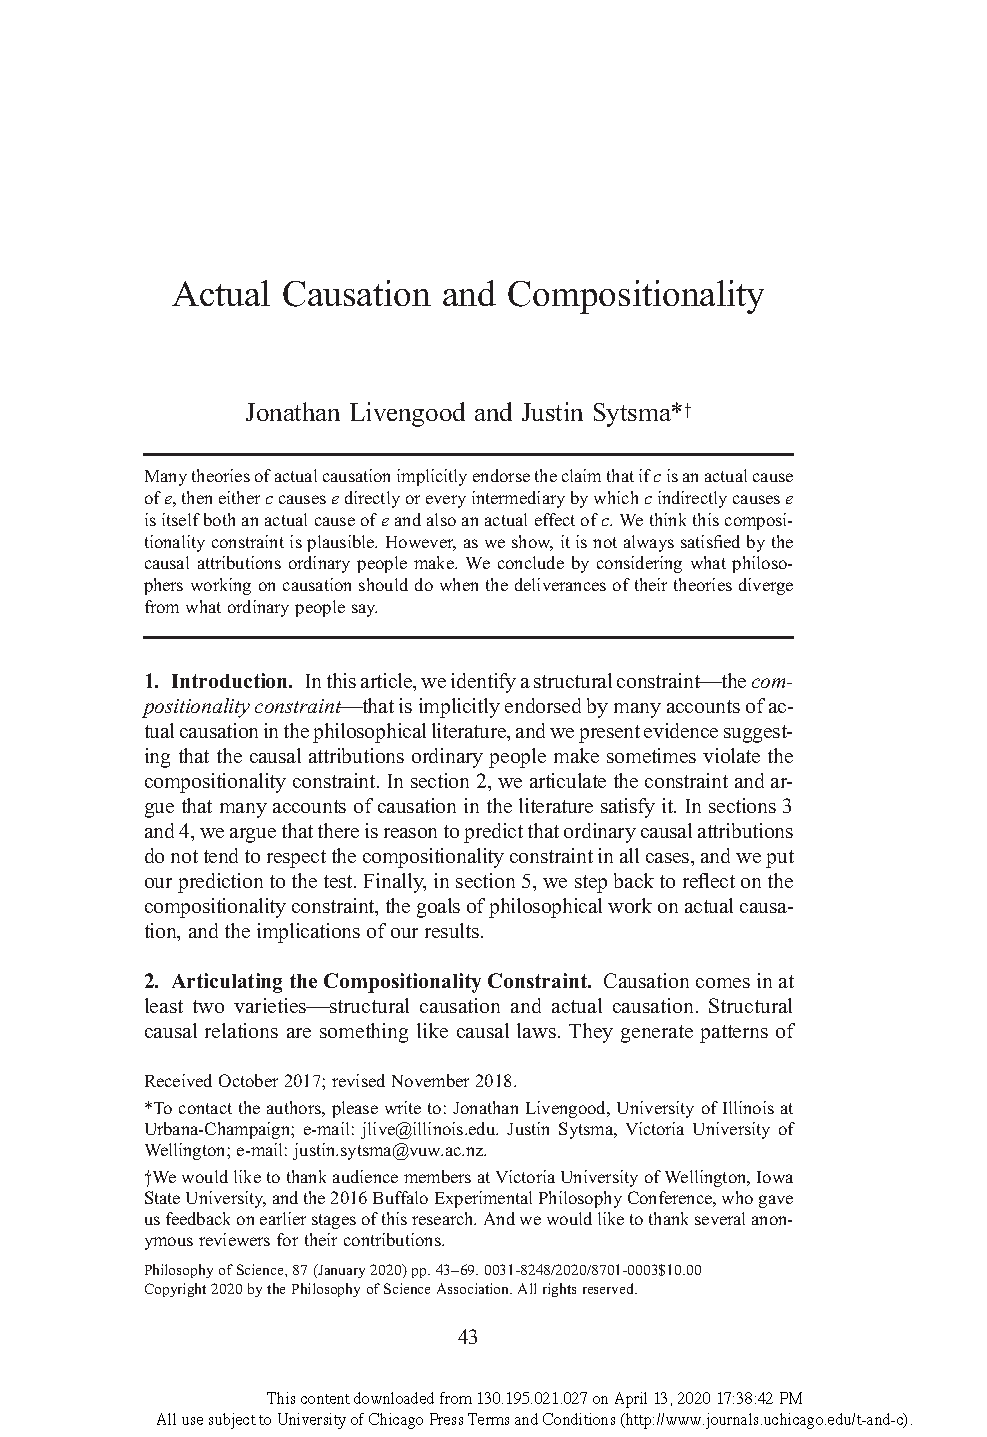
\includegraphics[width=\linewidth]{figures/livengood_sytsma_2020.pdf}}
   \frame{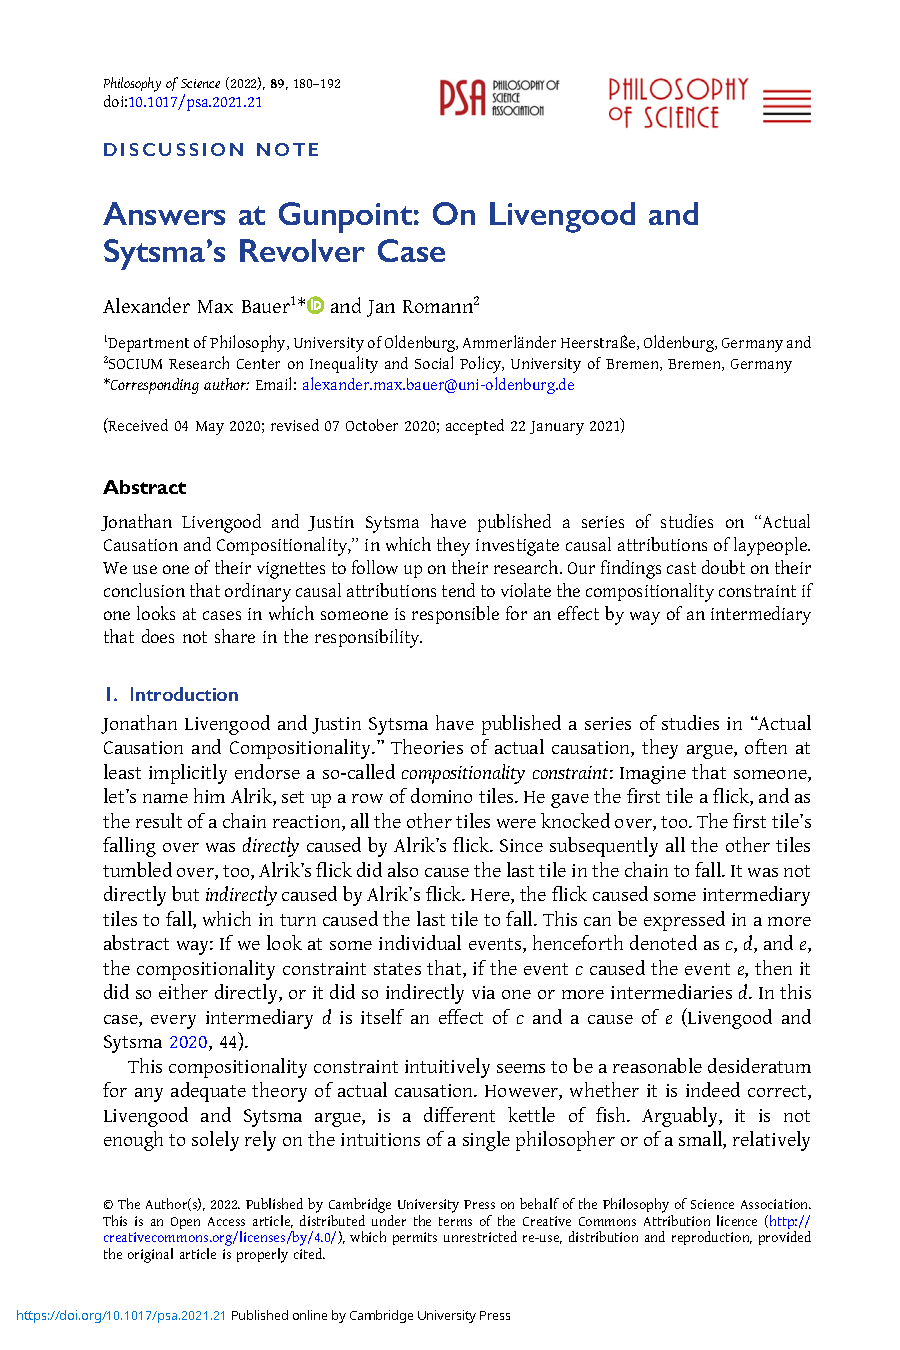
\includegraphics[width=\linewidth]{figures/bauer_romann_2022.pdf}}
   \frame{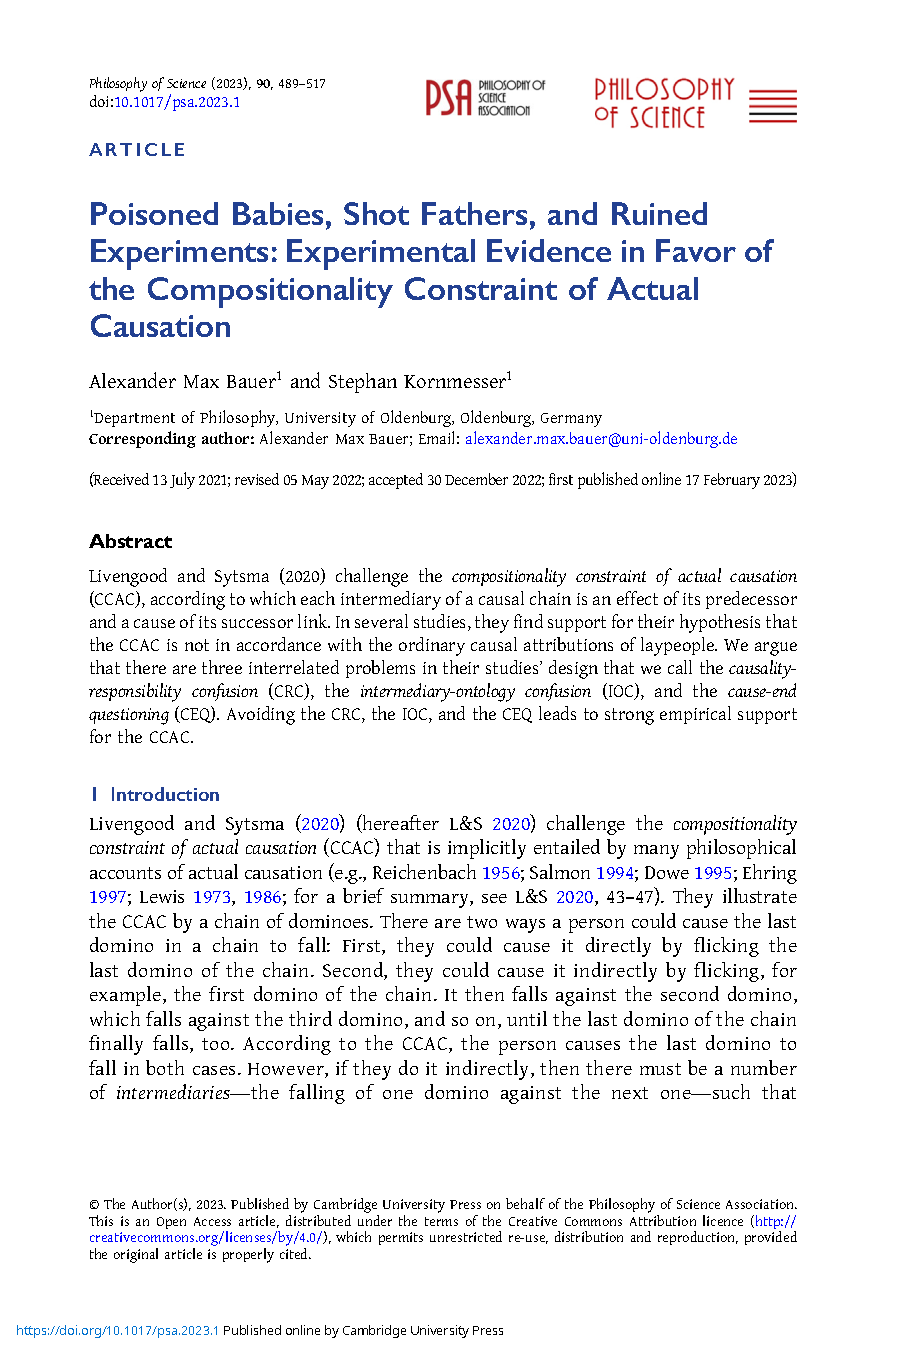
\includegraphics[width=\linewidth]{figures/bauer_kornmesser_2023.pdf}}
\end{center}
\end{multicols}
\note{
   \begin{itemize}
      \item all deal with concept of causation and how laypeople understand it
      \item focus on ``Compositionality Constraint'' or transitivity
   \end{itemize}
}
\end{frame}


%%%%%%%%%%%
% SLIDE 4 %
%%%%%%%%%%%
\begin{frame}{\vspace*{10mm}Livengood and Sytsma (2020): ``Actual Causation and Compositionality''}
\vspace*{-5mm}
\textbf{Compositionality Constraint of Actual Causation (CCAC):} If $c$ is an actual cause of $e$, then either $c$ causes $e$ directly, or every intermediary $d$ by which $c$ indirectly causes $e$ is itself an actual effect of $c$ and an actual cause of $e$. \textcolor{gray}{(Livengood and Sytsma 2020, p. 44)}
\begin{center}
   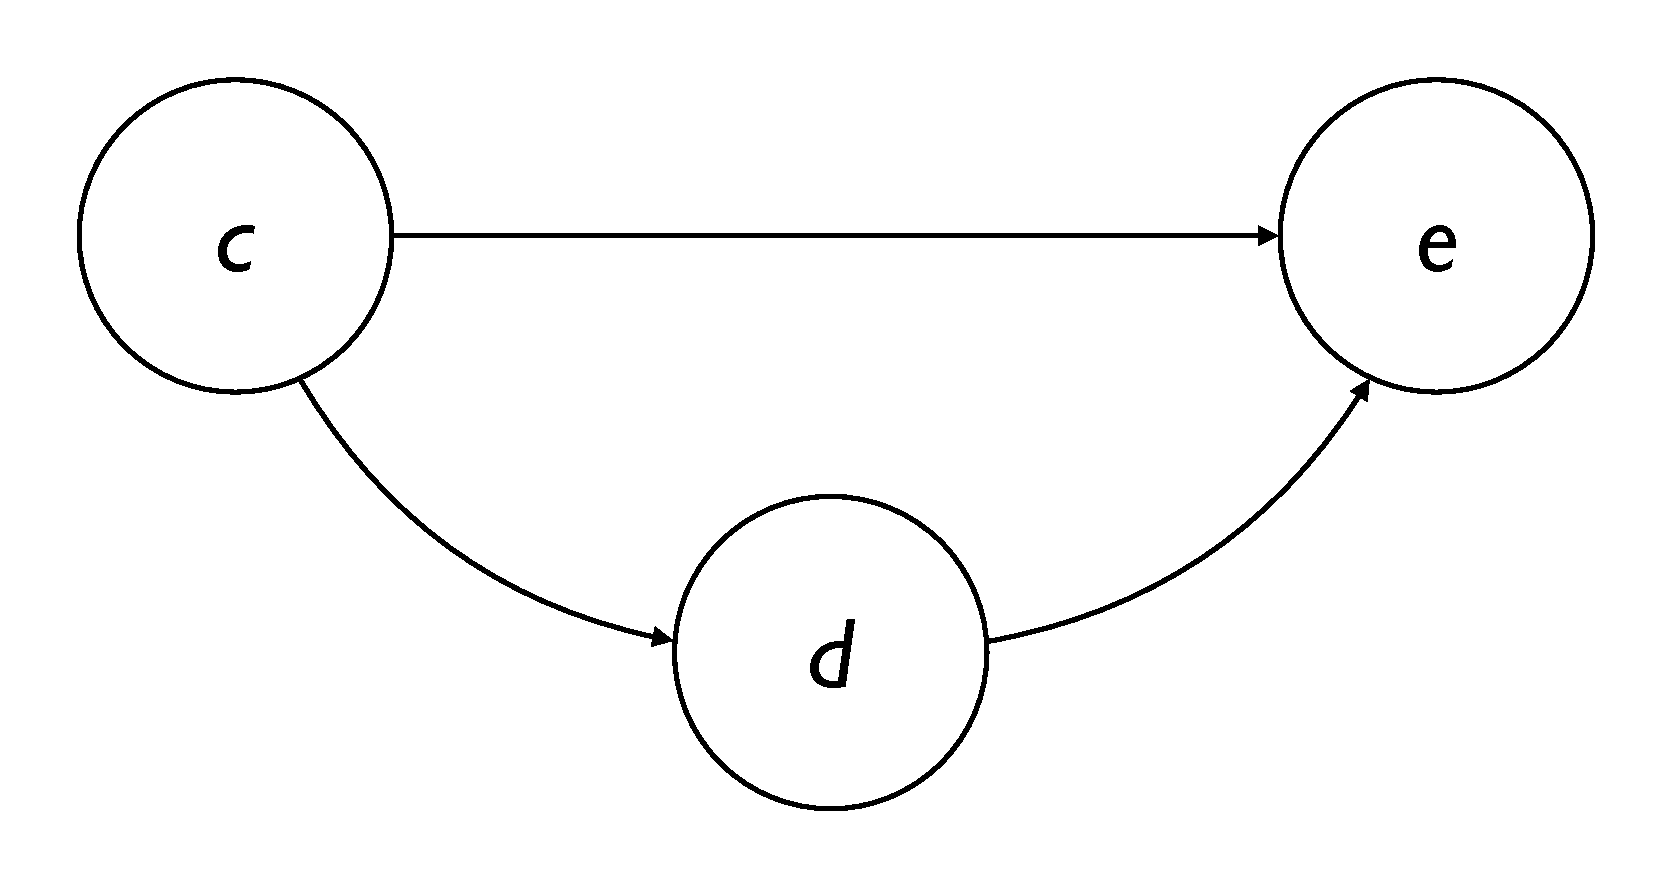
\includegraphics[width=0.5\linewidth]{figures/constraint.pdf}
\end{center}
\note{
   \begin{itemize}
      \item complex paper, only picking out some key elements
      \item at it's core concerned with the CCAC, compact definition of which is to be found on p. 44
      \item interested in how laypeople perceive the role/function of intermediaries ($d$)
   \end{itemize}
}
\end{frame}


%%%%%%%%%%%
% SLIDE 5 %
%%%%%%%%%%%
\begin{frame}{\vspace*{10mm}Livengood and Sytsma (2020): ``Actual Causation and Compositionality''}
\vspace*{-5mm}
\textbf{Poisoned Cup Vignette:} Amy wants to kill her daughter, Jessica, but she doesn't want to go to prison for murder. As such, Amy hatches a plan. She arranges for a babysitter, Courtney, to take care of Jessica while she is out of town on business. Before leaving, Amy laces one of Jessica's sippy cups with a deadly poison that is very difficult to detect. That evening, Courtney gives Jessica juice in the poisoned sippy cup. Jessica drinks the juice and dies two hours later. \textcolor{gray}{(Livengood and Sytsma 2020, p. 49)}
\begin{center}
   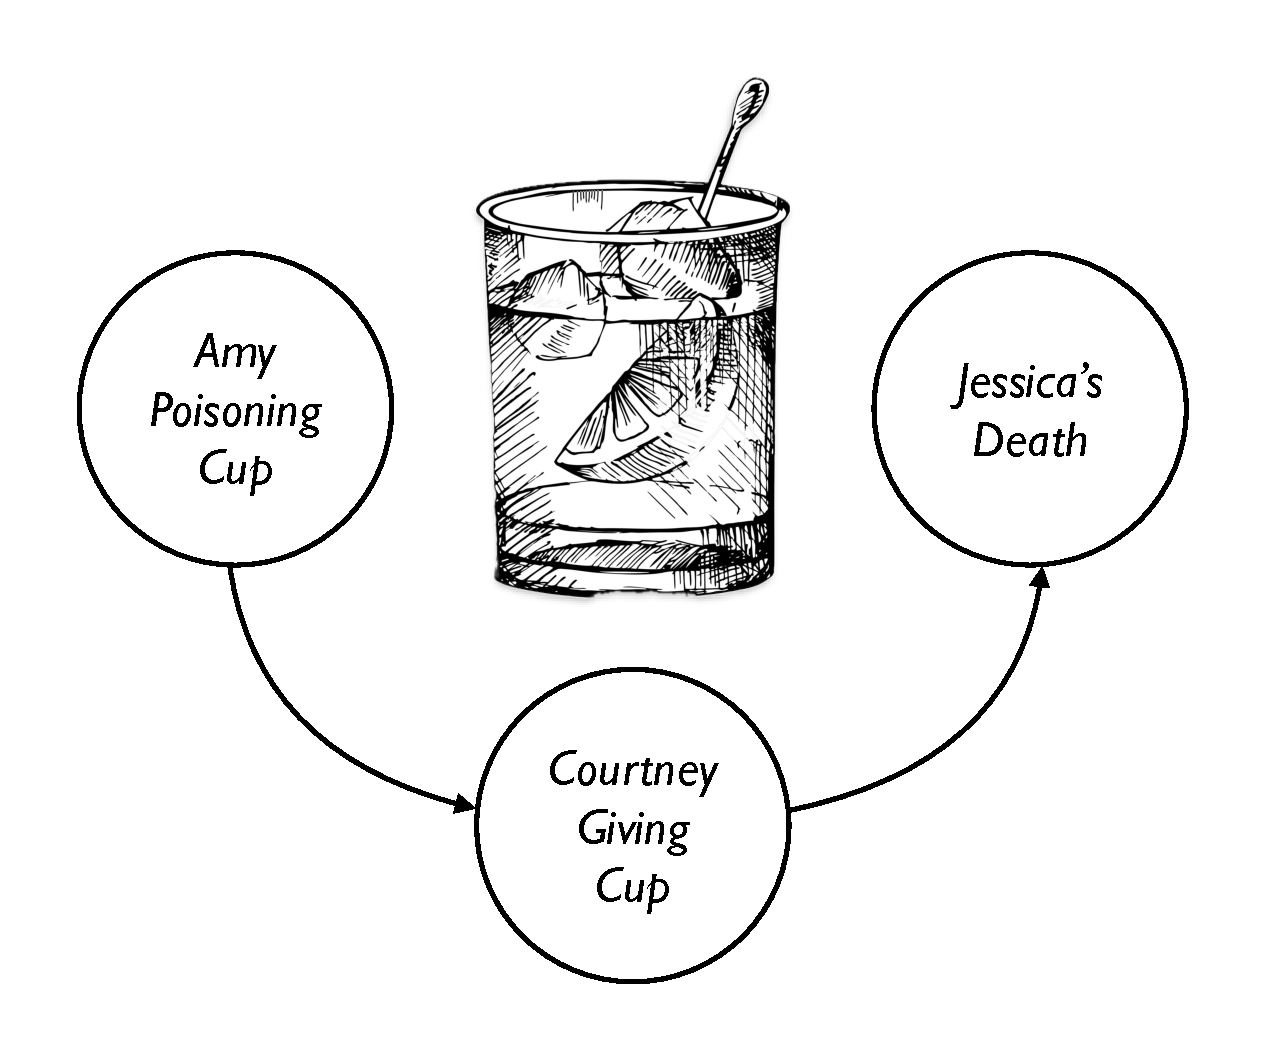
\includegraphics[width=0.3\linewidth]{figures/poison.pdf}
\end{center}
\note{
   \begin{itemize}
      \item to investigate, they use a number of vignettes
      \item presenting only three
      \item causal model for each is a chain
   \end{itemize}
}
\end{frame}


%%%%%%%%%%%
% SLIDE 6 %
%%%%%%%%%%%
\begin{frame}{\vspace*{10mm}Livengood and Sytsma (2020): ``Actual Causation and Compositionality''}
\vspace*{-5mm}
\begin{multicols}{2}
\textbf{Poisoned Cup Vignette}
\begin{itemize}
   \item $N=34$
   \item (dis)agreement on 7-point scale
   \item 2 statements
   \begin{itemize}
      \item[(A)] ``Amy caused Jessicas's death.''
      \item[(B)] ``Courtney caused Jessicas's death.''
   \end{itemize}
\end{itemize}
\vfill
\begin{center}
   \frame{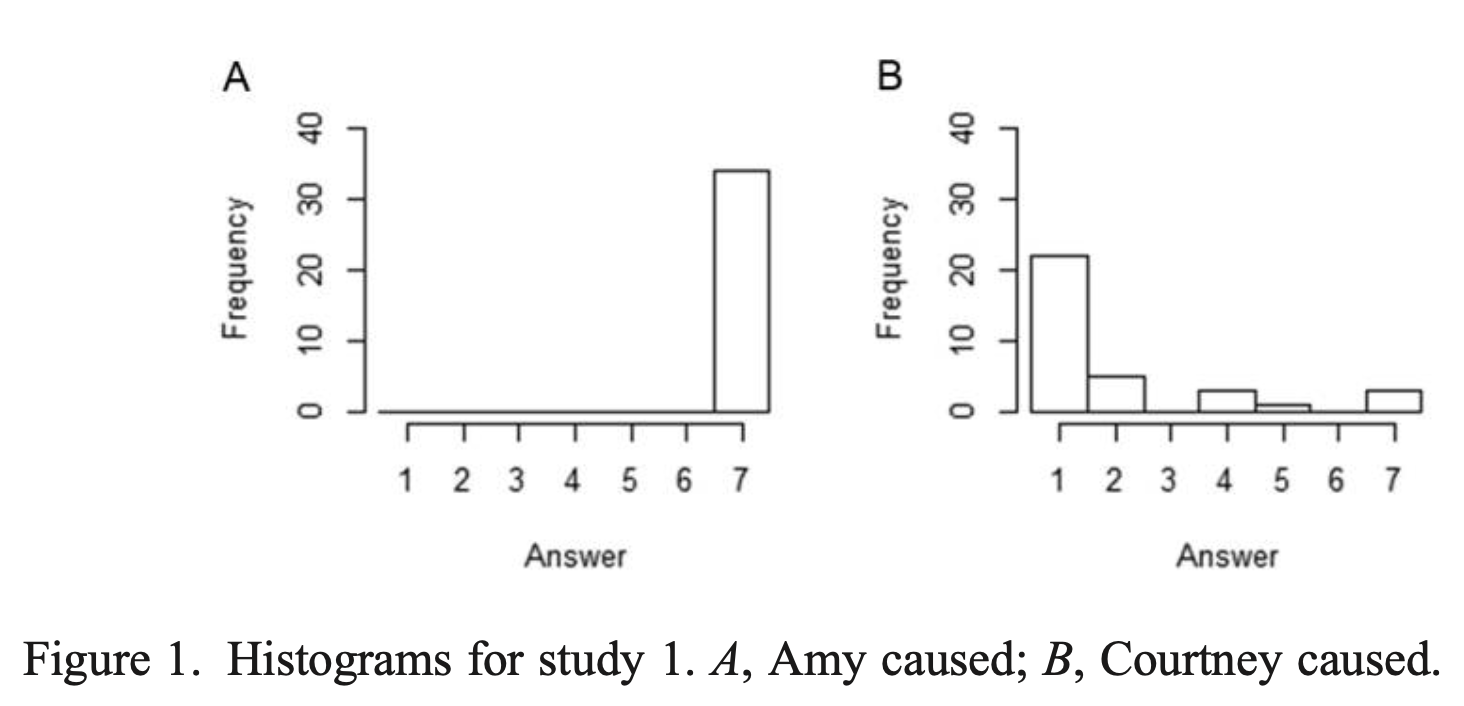
\includegraphics[width=\linewidth]{figures/livengood_sytsma_2020_fig_1.png}}
\end{center}
\end{multicols}
\note{
   \begin{itemize}
      \item each participant (34) completely agrees with (A)
      \item two-thirds of participants (22) completely disagree with (B)
      \item central tendency of responses is statistically significantly above/below 4 (neutral value, midpoint)
   \end{itemize}
}
\end{frame}


%%%%%%%%%%%
% SLIDE 7 %
%%%%%%%%%%%
\begin{frame}{\vspace*{10mm}Livengood and Sytsma (2020): ``Actual Causation and Compositionality''}
\vspace*{-5mm}
\textbf{Revolver Vignette:} Trent has decided to kill his father, Brad. He aims his loaded revolver at Brad and pulls the trigger, releasing the hammer. The hammer strikes the cartridge, igniting the gun powder. The gun powder explodes, driving the bullet from the gun. The bullet hits Brad in the head. He dies instantly. \textcolor{gray}{(Livengood and Sytsma 2020, p. 59)}
\begin{center}
   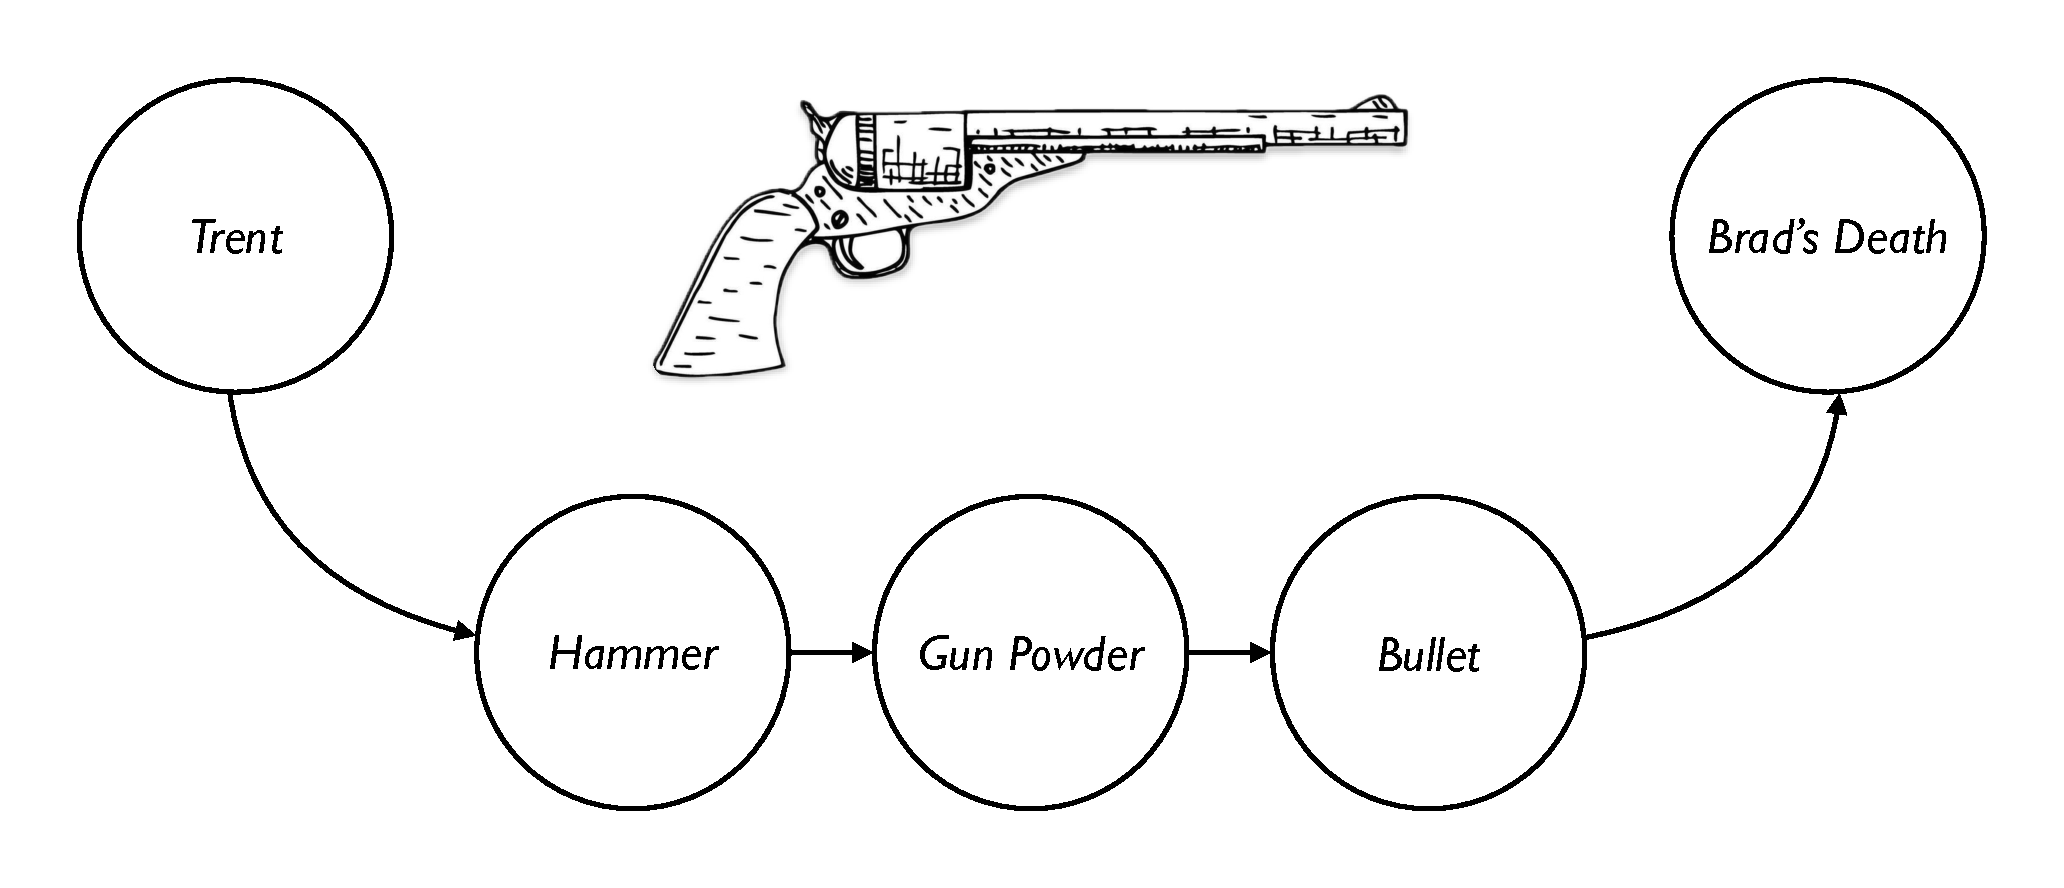
\includegraphics[width=0.75\linewidth]{figures/revolver_2.pdf}
\end{center}
\end{frame}


%%%%%%%%%%%
% SLIDE 8 %
%%%%%%%%%%%
\begin{frame}{\vspace*{10mm}Livengood and Sytsma (2020): ``Actual Causation and Compositionality''}
\vspace*{-5mm}
\begin{multicols}{2}
\textbf{Revolver Vignette}
\begin{itemize}
   \item $N=51$
   \item (dis)agreement on 7-point scale
   \item 4 statements
   \begin{itemize}
      \item[(A)] ``Trent caused Brad's death.''
      \item[(B)] ``The hammer caused Brad's death.''
      \item[(C)] ``The gun powder caused Brad's death.''
      \item[(D)] ``The bullet caused Brad's death.''
   \end{itemize}
\end{itemize}
\vfill
\begin{center}
   \frame{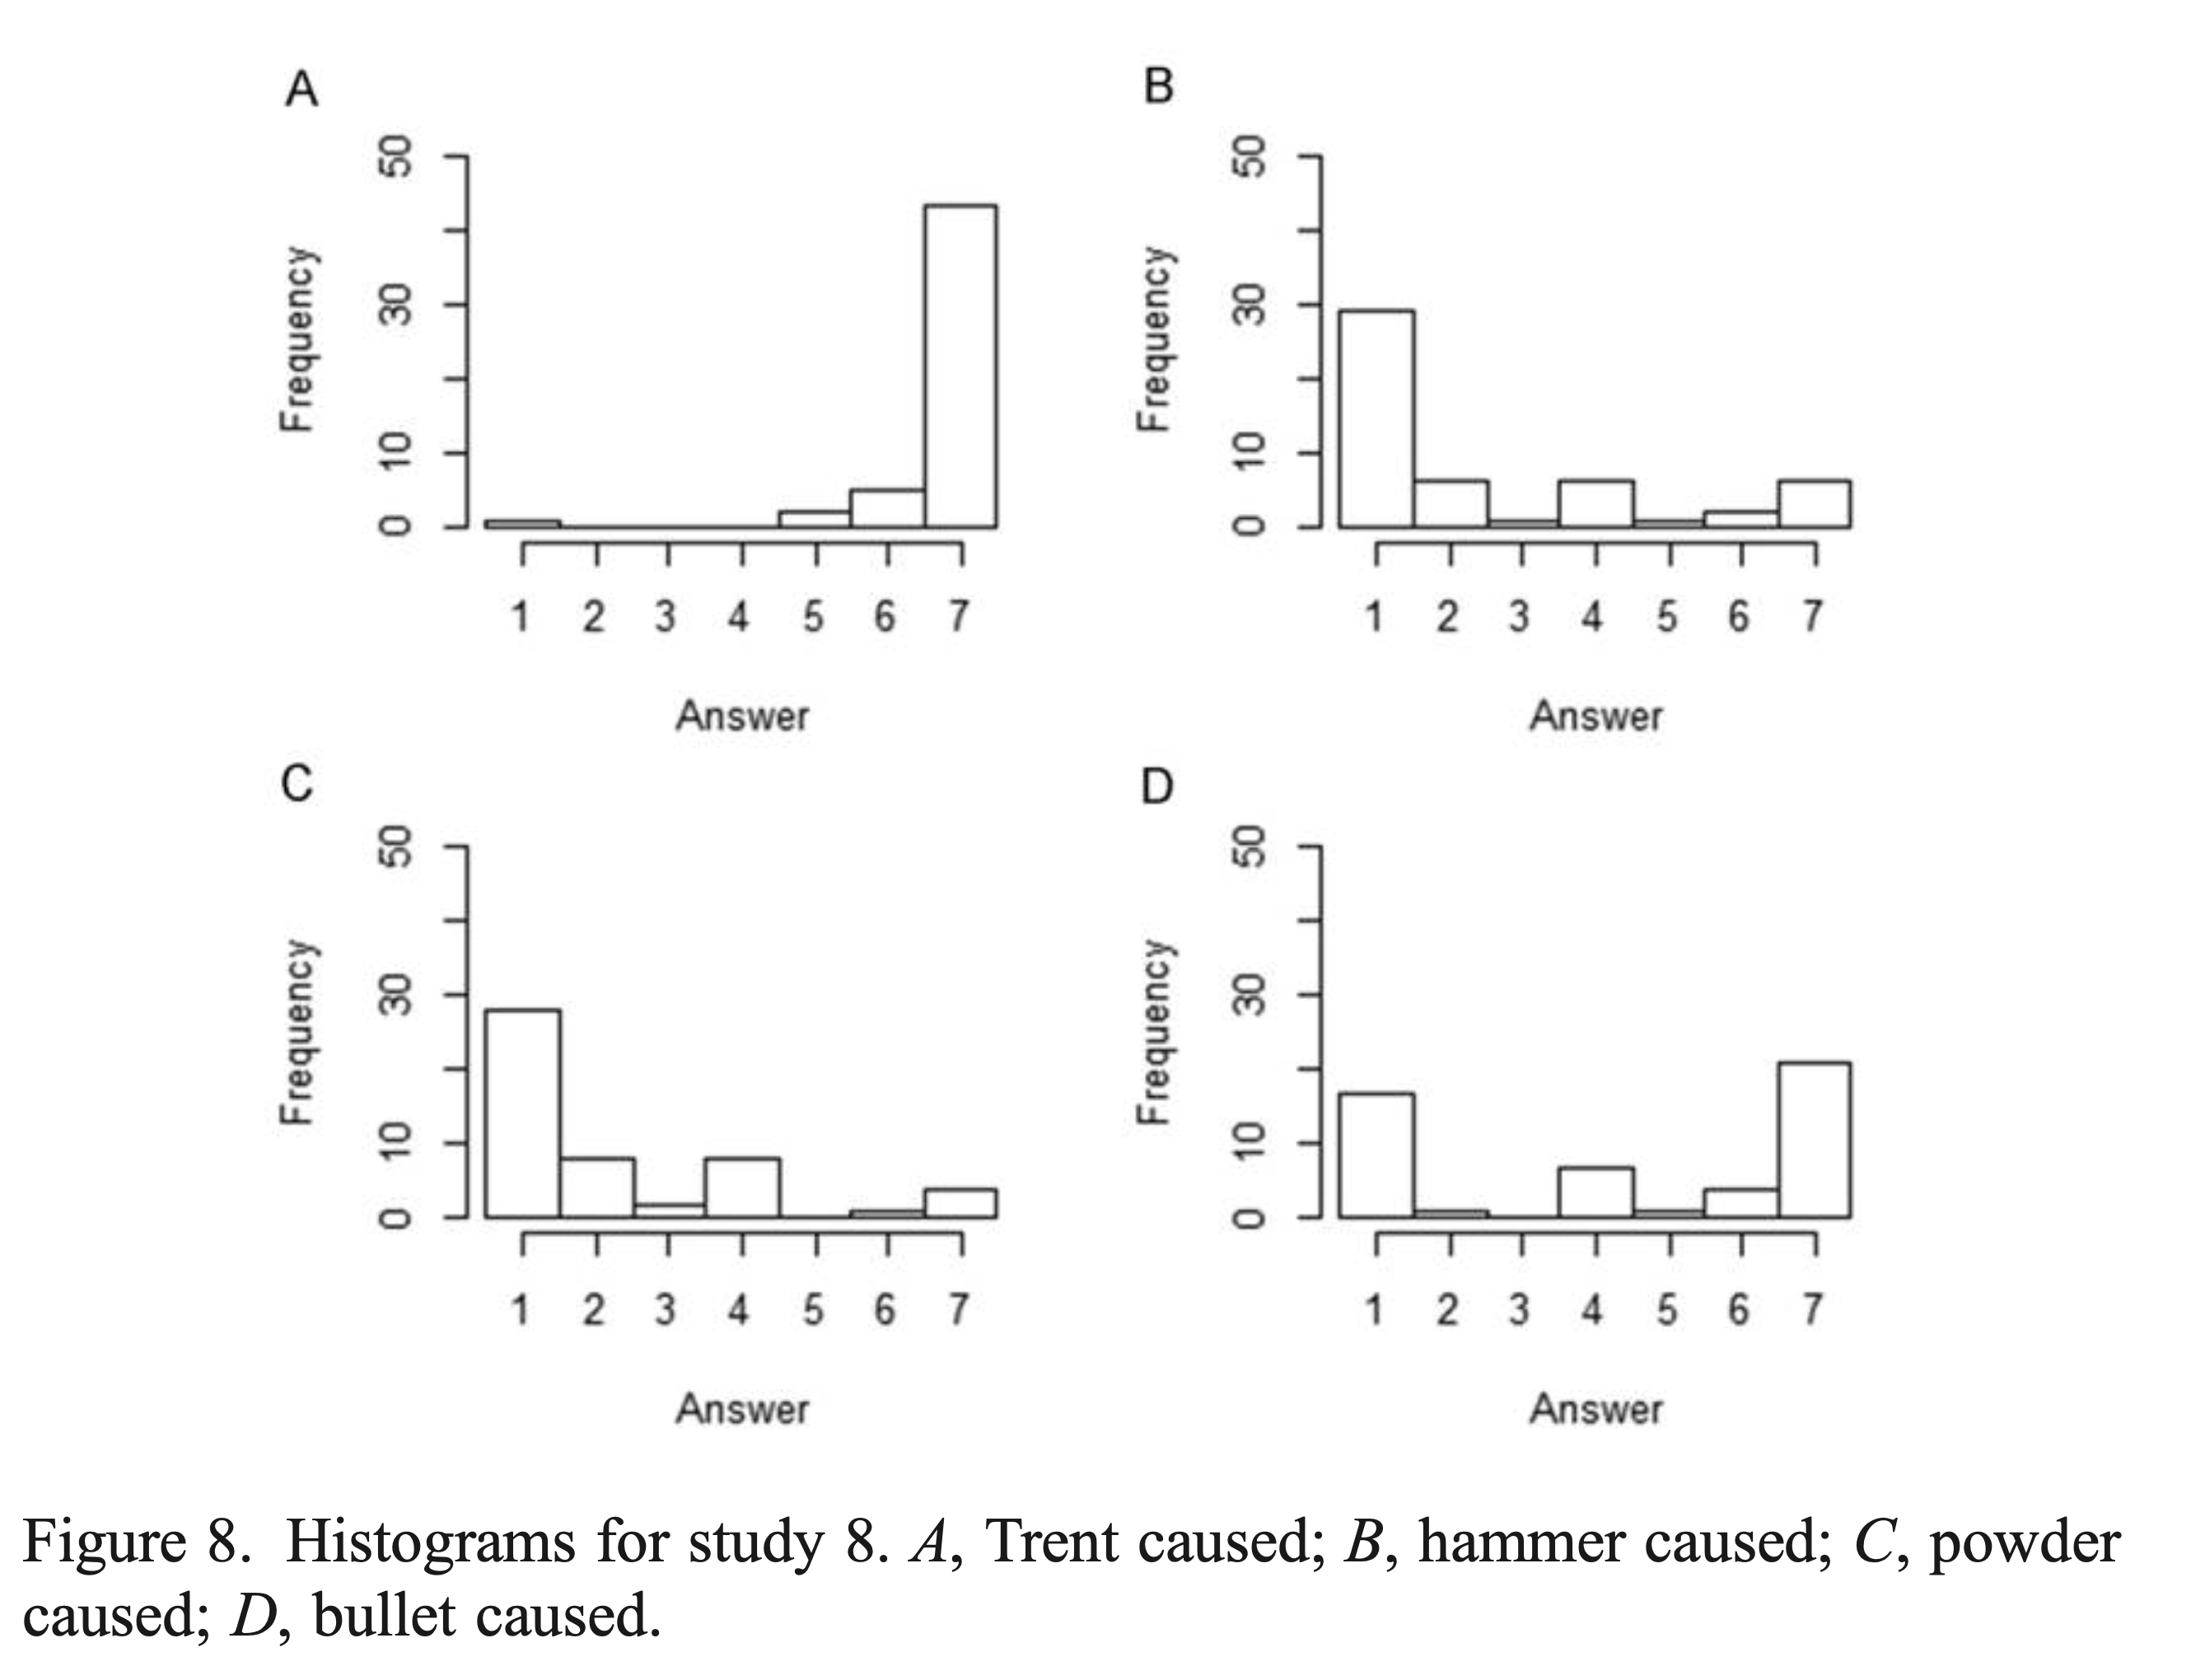
\includegraphics[width=\linewidth]{figures/livengood_sytsma_2020_fig_8.png}}
\end{center}
\end{multicols}
\note{
   \begin{itemize}
      \item 48 (nearly) completely agree with (A), choosing 6 or 7; central tendency of responses is statistically significantly above 4
      \item not so for (B) and (C), where central tendency is significantly below 4
      \item assessments of (D) were bimodal; central tendency not statistically different from 4
   \end{itemize}
}
\end{frame}


%%%%%%%%%%%
% SLIDE 9 %
%%%%%%%%%%%
\begin{frame}{\vspace*{10mm}Livengood and Sytsma (2020): ``Actual Causation and Compositionality''}
\vspace*{-5mm}
\textbf{GFCI Vignette:} John is a scientist conducting a very important experiment on an unusual species of plant. His experiment requires growing his plants under a special light, which is plugged into an outlet with a ground fault circuit interrupter (GFCI) safety mechanism. The pipes running to John's laboratory were correctly manufactured and installed, and the system was protected from any changes in weather condition.\par
\hspace{2em}Despite there being nothing wrong with the pipes, one day a pipe burst in John's laboratory. Water ran into the outlet powering the special light. A properly functioning GFCI safety mechanism will break the circuit so that no power flows through its outlet if exposed to water in this way. And in fact, the GFCI safety mechanism did break the circuit. The special light turned off and the experiment was ruined. \textcolor{gray}{(Livengood and Sytsma 2020, p. 62)}
\begin{center}
   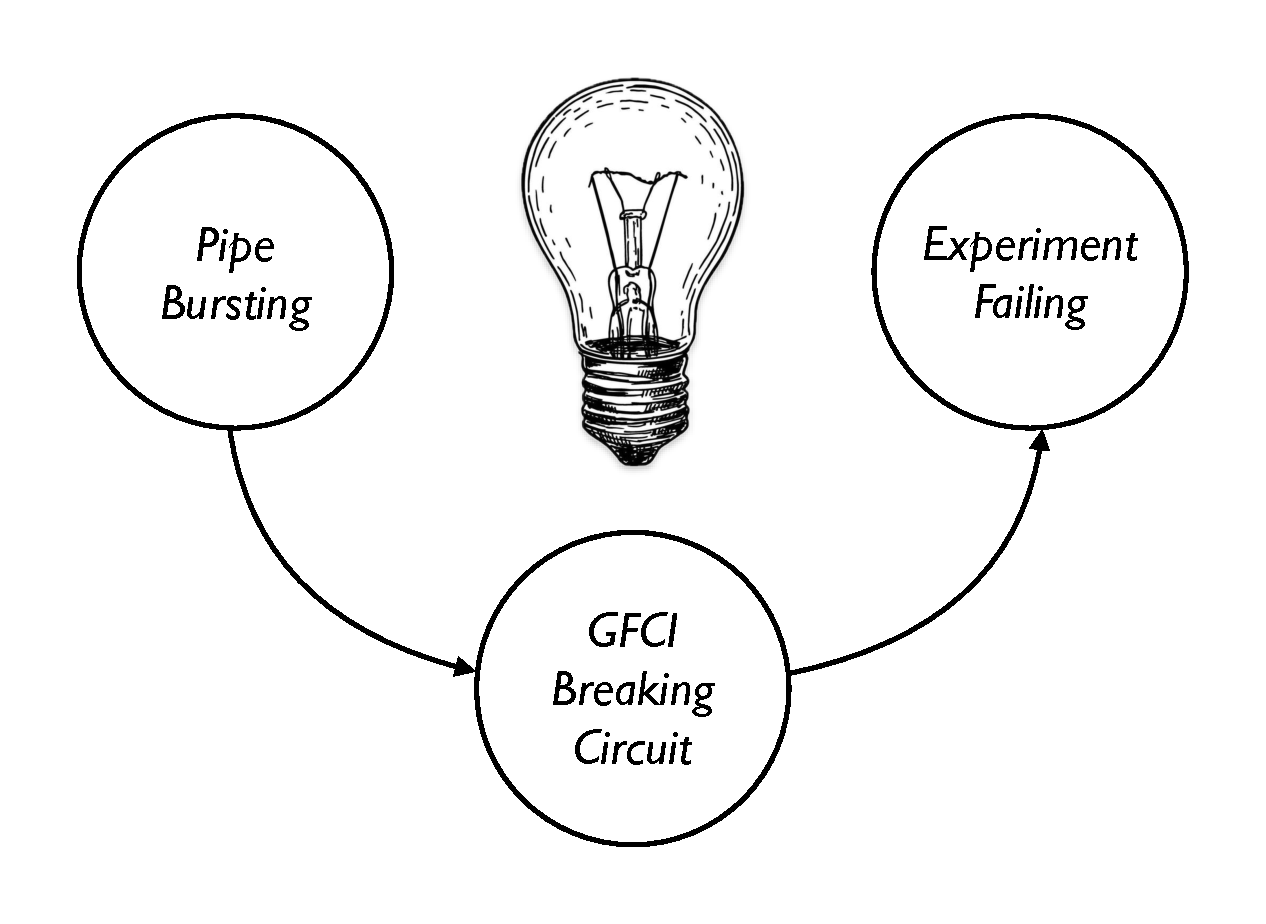
\includegraphics[width=0.2\linewidth]{figures/gfci.pdf}
\end{center}
\end{frame}


%%%%%%%%%%%%
% SLIDE 10 %
%%%%%%%%%%%%
\begin{frame}{\vspace*{10mm}Livengood and Sytsma (2020): ``Actual Causation and Compositionality''}
\vspace*{-5mm}
\begin{multicols}{2}
\textbf{GFCI Vignette}
\begin{itemize}
   \item $N=163$
   \item (dis)agreement on 7-point scale
   \item 2 statements
   \begin{itemize}
      \item[(A)] ``The pipe caused the experiment to be ruined.''
      \item[(B)] ``The GFCI caused the experiment to be ruined.''
   \end{itemize}
\end{itemize}
\vfill
\begin{center}
   \frame{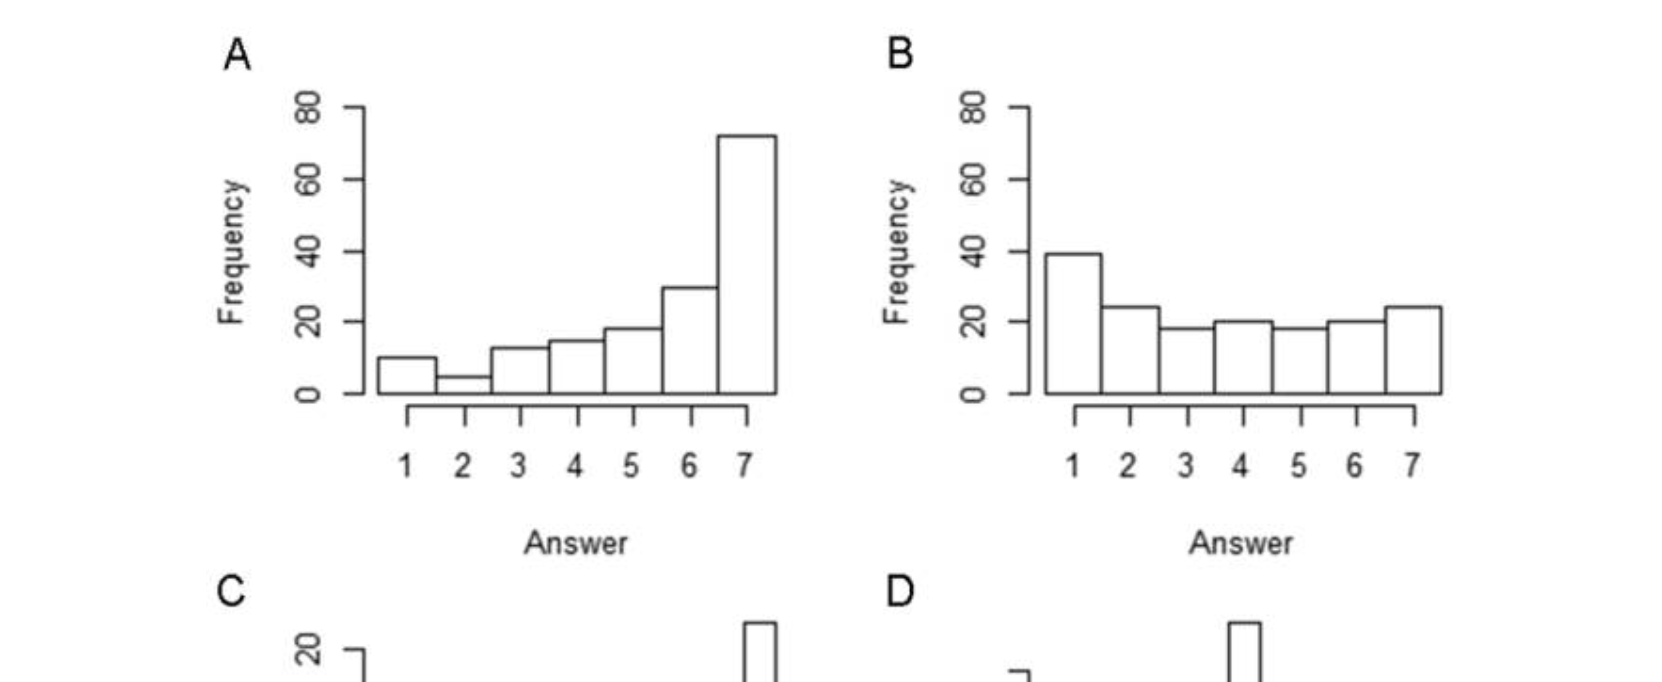
\includegraphics[width=\linewidth]{figures/livengood_sytsma_2020_fig_9_1.png}}
   \frame{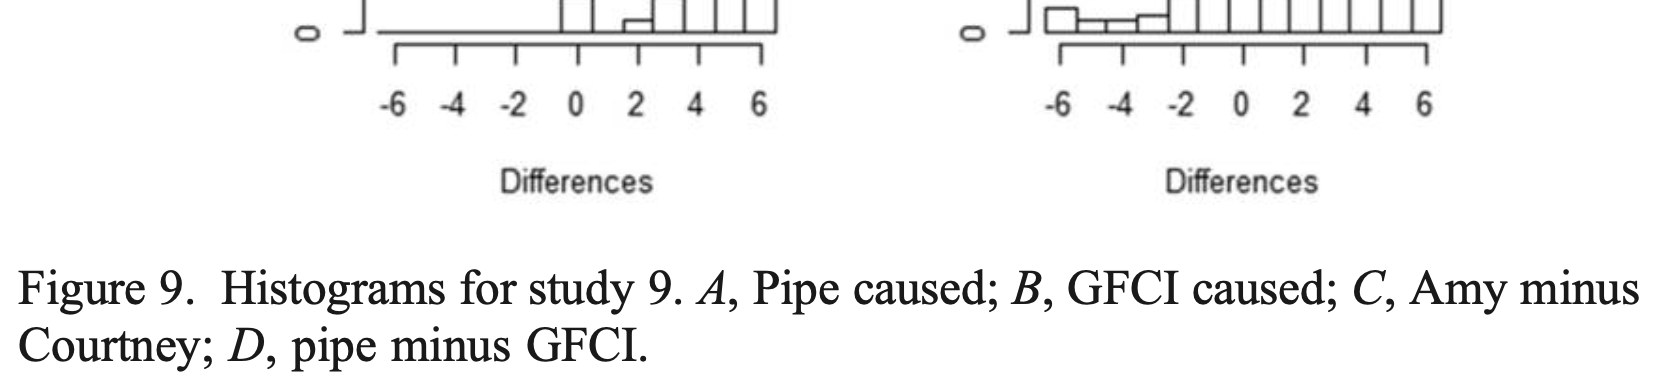
\includegraphics[width=\linewidth]{figures/livengood_sytsma_2020_fig_9_2.png}}
\end{center}
\end{multicols}
\note{
   \begin{itemize}
      \item 72 participants completely agree with (A), another 30 respond with 6
      \item central tendency of responses is statistically significantly above/below 4
      \item hence, CCAC violated; intermediaries by which effect is caused indirectly are not deemed to be an actual actual cause of $e$
   \end{itemize}
}
\end{frame}


%%%%%%%%%%%%
% SLIDE 11 %
%%%%%%%%%%%%
\begin{frame}{\vspace*{10mm}Bauer and Romann (2022): ``Answers at Gunpoint''}
\vspace*{-5mm}
\begin{multicols}{2}
\textbf{Events}\\
8 different events
\begin{itemize}
   \item[(A)] ``pulling the trigger''
   \item[(B)] ``releasing the hammer''
   \item[(C)] ``striking the cartridge''
   \item[(D)] ``igniting the gun powder''
   \item[(E)] ``the gun powder exploding''
   \item[(F)] ``driving the bullet from the gun''
   \item[(G)] ``the bullet hitting Brad in the head''
   \item[(H)] ``the death of Brad''
\end{itemize}
\vfill
\begin{center}
   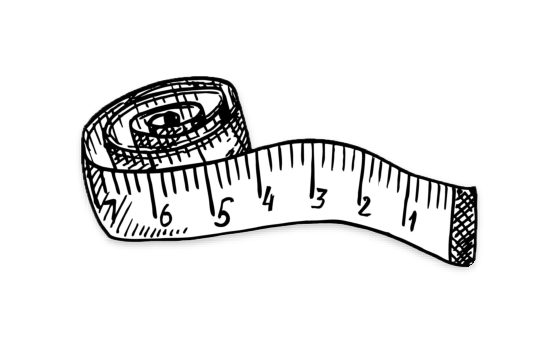
\includegraphics[width=\linewidth]{figures/tape_measure.pdf}
\end{center}
\end{multicols}
\note{
   \begin{itemize}
      \item struck me as odd that there is a whole lot of statements about causation to be made from the vignettes used, but only a small hand full of them was presented
      \item Jan Romann and I wanted to know whether this \textit{selection} of statements might have an effect on results
   \end{itemize}
}
\end{frame}


%%%%%%%%%%%%
% SLIDE 12 %
%%%%%%%%%%%%
\begin{frame}{\vspace*{10mm}Bauer and Romann (2022): ``Answers at Gunpoint''}
\vspace*{-5mm}
\textbf{Combinations of events}\\
28 ``X caused Y'' statements, e.\,g.,
\begin{itemize}
   \item[(A/B)] ``Pulling the trigger caused the release of the hammer.''
   \item[(C/D)] ``Striking the cartridge caused the ignition of the gun powder.''
   \item[(F/G)] ``The bullet being driven from the gun caused the bullet to hit Brad in the head.''
\end{itemize}
\hfill
\begin{center}
   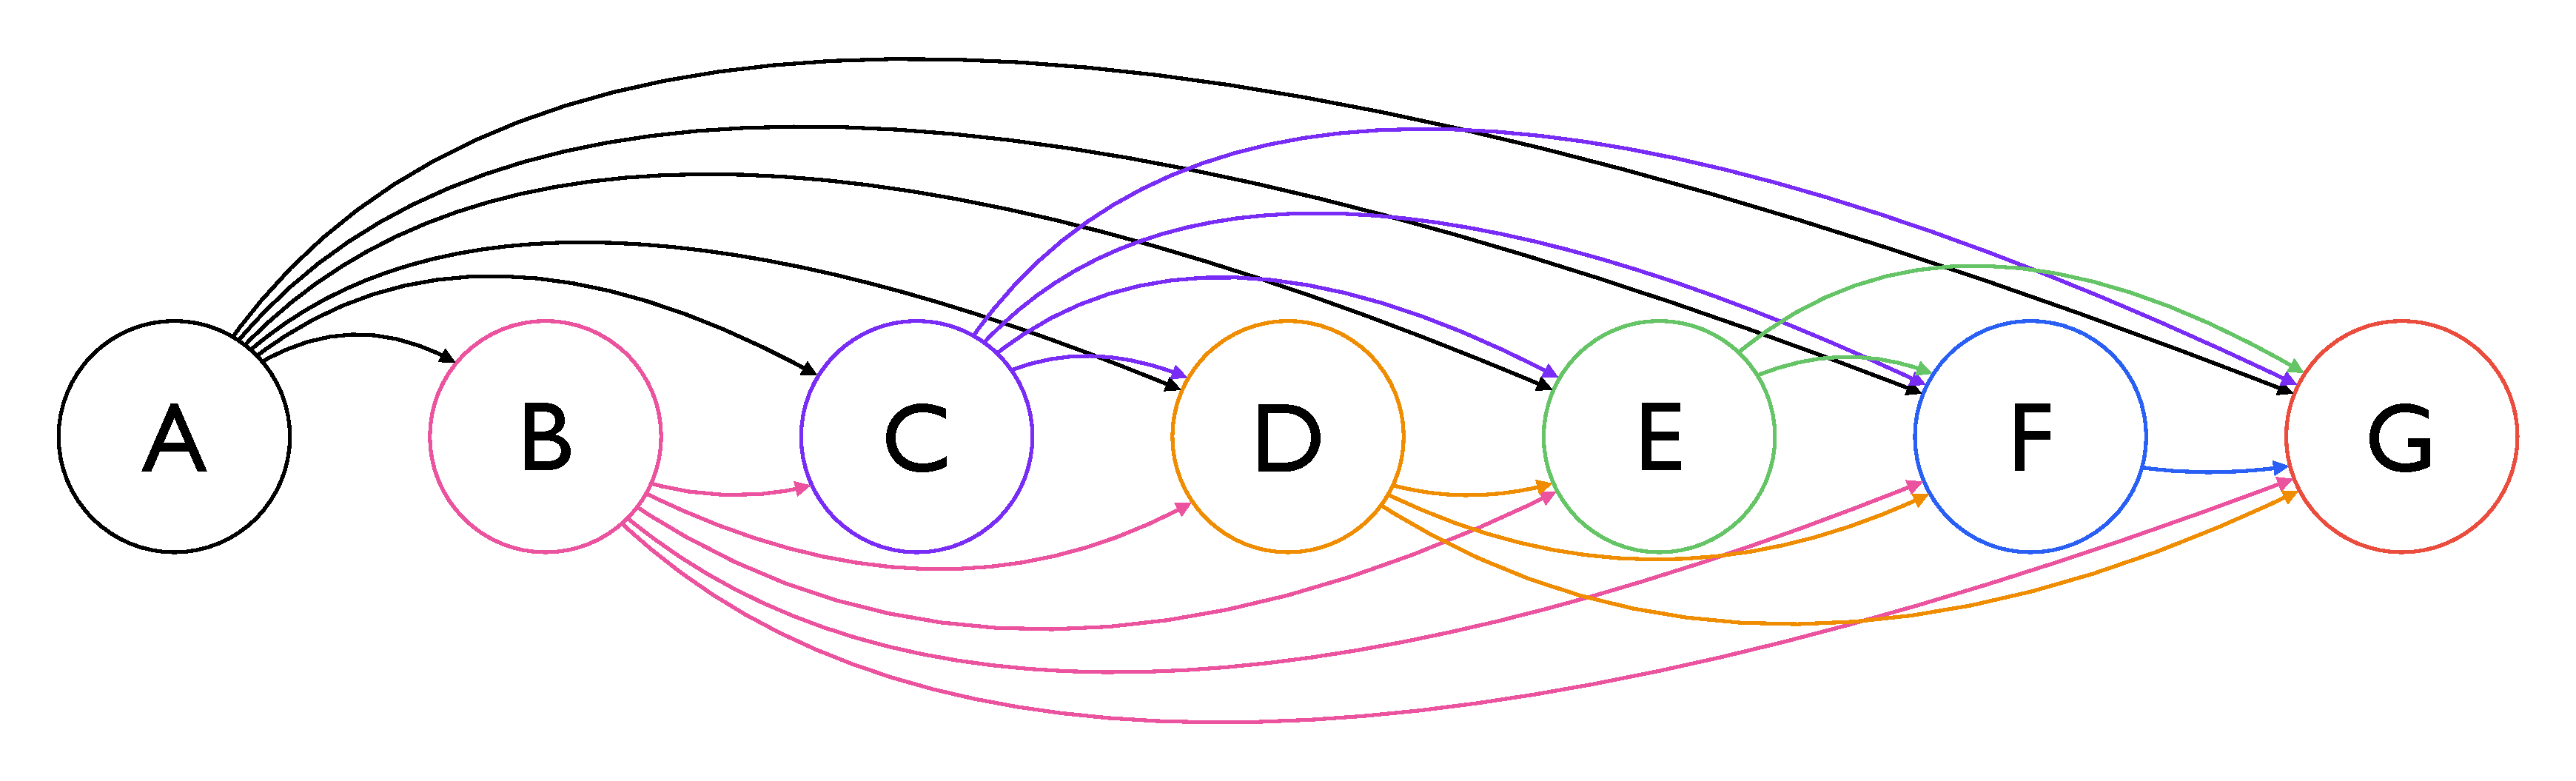
\includegraphics[width=.8\linewidth]{figures/combinations.pdf}
\end{center}
\note{
   \begin{itemize}
      \item sum of all forward facing combinations to be made of the events
      \item my, by that time vague, idea about this: albeit LS tried to avoid this, the selected statements led subjects to think about causation in terms of responsibility
      \item one way to counter this, could be to include statements that are clearly free from moral baggage, as, e.\,g., ``Releasing the hammer caused the hammer to strike the cartridge.''
   \end{itemize}
}
\end{frame}


%%%%%%%%%%%%
% SLIDE 13 %
%%%%%%%%%%%%
\begin{frame}{\vspace*{10mm}Bauer and Romann (2022): ``Answers at Gunpoint''}
\vspace*{-5mm}
\textbf{(More or Less) Analogous Statements}\\
\begin{itemize}
   \item[(1)] ``Trent caused Brad's death.''
   \item[(A/H)] ``Pulling the trigger caused the death of Brad.''
\end{itemize}
\vspace*{0.5em}
\begin{itemize}
   \item[(2)] ``The hammer caused Brad's death.''
   \item[(B/H)] ``Releasing the hammer caused the death of Brad.''
\end{itemize}
\vspace*{0.5em}
\begin{itemize}
   \item[(3)] ``The gun powder caused Brad's death.''
   \item[(D/H)] ``Igniting the gun powder caused the death of Brad.''
   \item[(E/H)] ``The explosion of the gun powder caused the death of Brad.''
\end{itemize}
\vspace*{0.5em}
\begin{itemize}
   \item[(4)] ``The bullet powder caused Brad's death.''
   \item[(F/H)] ``The bullet being driven from the gun caused the death of Brad.''
   \item[(G/H)] ``The bullet hitting Brad in the head caused the death of Brad.''
\end{itemize}
\note{
   \begin{itemize}
      \item to see if this makes a difference, have had to include statements that are similar
      \item due to method of construction, ended up with slightly different formulations, but considered the following to be (more or less) similar
   \end{itemize}
}
\end{frame}


%%%%%%%%%%%%
% SLIDE 14 %
%%%%%%%%%%%%
\begin{frame}{\vspace*{10mm}Bauer and Romann (2022): ``Answers at Gunpoint''}
\vspace*{-5mm}
\begin{multicols}{2}
\textbf{Results}\\
\begin{itemize}
   \item $N=52$
   \item (dis)agreement on 7-point scale
   \item 28 statements
   \item central tendency for no statement smaller than the ``neutral'' value 4
\end{itemize}
\vfill
\begin{center}
   \frame{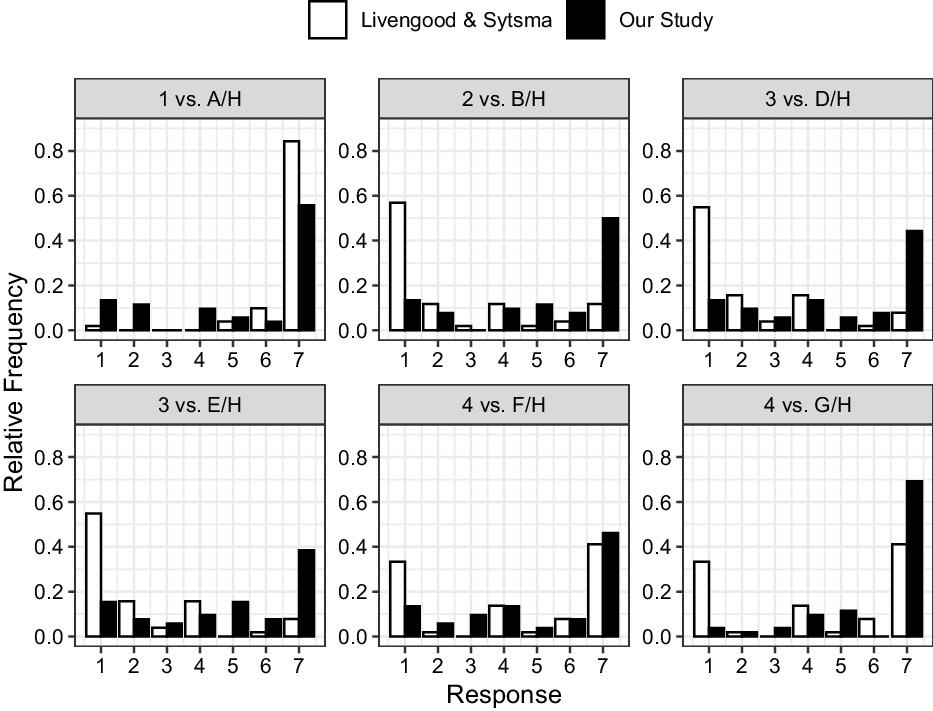
\includegraphics[width=\linewidth]{figures/bauer_romann_2020_fig_1.png}}
\end{center}
\end{multicols}
\note{
   \begin{itemize}
      \item Wilcoxon matched-pairs signed-rank tests (corrected p-values) reject the hypothesis that the central tendency for any of the 28 statements is smaller than or equal to 4
      \item when questioning people, we must be very careful not only in choosing our words but also in choosing our sets of questions
      \item does not tell much about where these differences might come from
   \end{itemize}
}
\end{frame}


%%%%%%%%%%%%
% SLIDE 15 %
%%%%%%%%%%%%
\begin{frame}{\vspace*{10mm}Bauer and Kornmesser (2023): ``Poisoned Babies, Shot Fathers, and Ruined Experiments''}
\vspace*{-5mm}
\textbf{Causation--Responsibility Confusion:} In ``x caused y'' statements, the verb ``cause'' is ambiguous and might be understood in moral terms \textcolor{gray}{(also see Samland and Waldmann 2014)}\\
\vspace*{1em}
\textbf{Intermediary--Ontology Confusion:} Typically, events are the relata of causal chains, not agents or objects. Using agents or objects leads people to understand the verb ``cause'' in moral terms. \textcolor{gray}{(also see Samland and Waldmann 2016)}\\
\vspace*{1em}
\textbf{Cause-End Questioning:} If, in ``x caused y'' statements, y is always the end point of a causal chain, this emphasises the end point. If the end point is of moral significane, this might lead subjects to view the statements in moral terms \textcolor{gray}{(also see Bauer and Romann 2022)}\\
\vfill
\note{
   \begin{itemize}
      \item 3 possible reasons for differences
      \item closely interrelated
   \end{itemize}
}
\end{frame}


%%%%%%%%%%%%
% SLIDE 16 %
%%%%%%%%%%%%
\begin{frame}{\vspace*{10mm}Bauer and Kornmesser (2023): ``Poisoned Babies, Shot Fathers, and Ruined Experiments''}
\vspace*{-5mm}
\textbf{Design}\\
\begin{itemize}
   \item $N\approx 60$ for each study (16 studies in total)
   \item (dis)agreement on 7-point scale
   \item vignettes from Livengood and Sytsma (2020)
      \begin{itemize}
         \item poisoned cup vignette
         \item revolver vignette
         \item GFCI vignette
      \end{itemize}
   \item studies for each vignette
      \begin{itemize}
         \item replication
         \item exclusion of IOC
         \item exclusion of CRC
         \item exclusion of CEQ
         \item simultaneous exclusion of IOC, CRC, and CEQ
      \end{itemize}
\end{itemize}
\vfill
\note{
   \begin{itemize}
      \item \textbf{Causation-Responsibility Confusion:} not using the word ``cause''
      \item \textbf{Intermediary-Ontology Confusion:} using events instead of individuals as intermediaries
      \item \textbf{Cause-End Questioning:} using statements in which an intermediary $d_1$ is the cause of an effect that is not the end link of the causal chain but a further intermediary $d_2$
   \end{itemize}
}
\end{frame}


%%%%%%%%%%%%
% SLIDE 17 %
%%%%%%%%%%%%
\begin{frame}{\vspace*{10mm}Bauer and Kornmesser (2023): ``Poisoned Babies, Shot Fathers, and Ruined Experiments''}
\vspace*{-5mm}
\textbf{Results}\\
\begin{itemize}
   \item successful replication \textcolor{gray}{(for all vignettes)}
   \item excluding IOC led to less disagreement that intermediaries are causes \textcolor{gray}{(for poisoned cup and revolver vignette)}
   \item excluding CRC led to agreement that intermediaries are causes \textcolor{gray}{(for poisoned cup and revolver vignette)}
   \item excluding CEQ led to agreement that intermediaries are causes \textcolor{gray}{(for all vignettes)}
   \item simultaneous exclusion of IOC, CRC, and CEQ led to agreement that intermediaries are causes \textcolor{gray}{(for all vignettes)}
\end{itemize}
\vfill
\end{frame}


%%%%%%%%%%%%
% SLIDE 18 %
%%%%%%%%%%%%
\begin{frame}{\vspace*{10mm}Takeaway Points}
\vspace*{-5mm}
\textbf{Key Assumptions in Light of the Data}
\begin{itemize}
   \item if asked the right way, subjects can be prevented from confusing causation with responsibility
   \item subjects' intuitions are not in conflict with the Compositionality Constraint of Actual Causation \textcolor{gray}{(contrary to Livengood and Sytsma 2020)}
   \item responsibility might not be (such a large) part of the concept of causation \textcolor{gray}{(contrary to proponents of the \textit{responsibility view})}
\end{itemize}
\vfill
\end{frame}


%%%%%%%%%%%%
% SLIDE 19 %
%%%%%%%%%%%%
\begin{frame}{}
\begin{center}
   {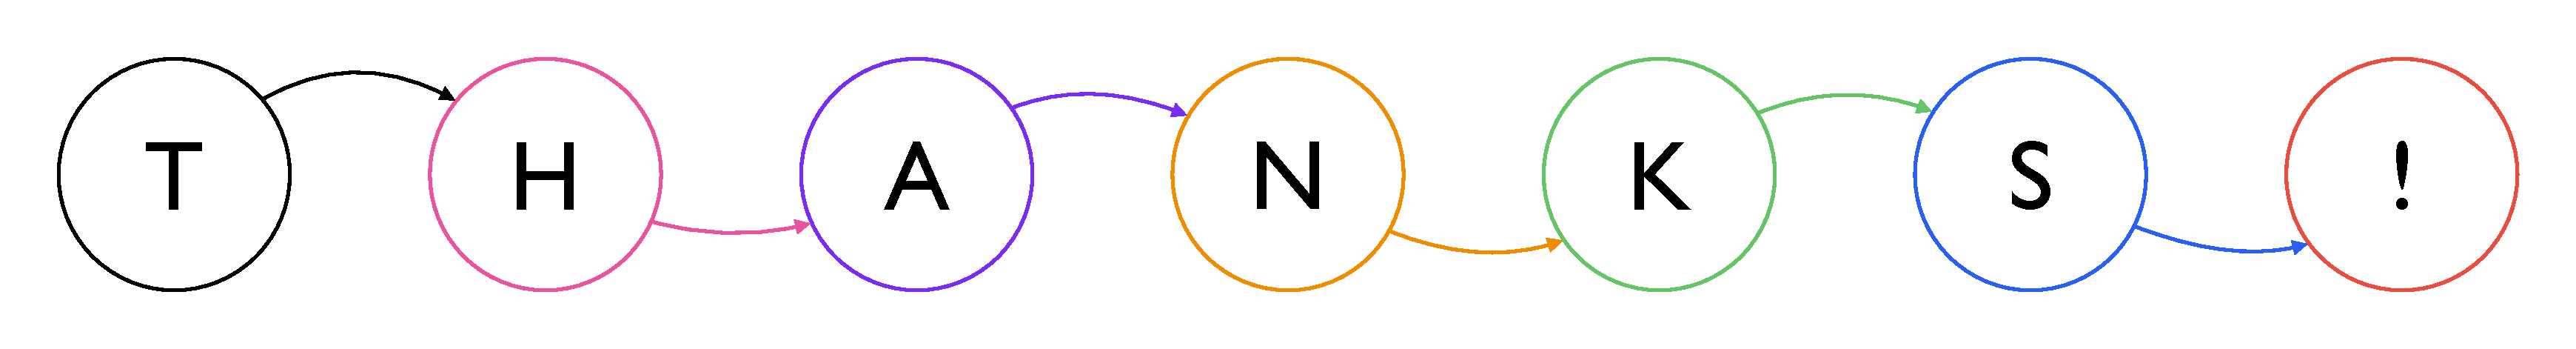
\includegraphics[width=0.9\linewidth]{figures/thanks.pdf}}
\end{center}
{\footnotesize
\textbf{Data}\\
https://github.com/alephmembeth/causality-revolver\\
https://github.com/alephmembeth/causality-compositionality\\
\vspace{0.5em}
\textbf{References}\\
\vspace{-0.5em}
\begin{itemize}[label=,leftmargin=2em,itemindent=-2em]
   \item Bauer, Alexander Max, and Stephan Kornmesser (2023): ``Poisoned Babies, Shot Fathers, and Ruined Experiments. Experimental Evidence in Favor of the Compositionality Constraint of Actual Causation''. \textit{Philosophy of Science} 90, 489--517.
   \item Bauer, Alexander Max, and Jan Romann (2022): ``Answers at Gunpoint. On Livengood and Sytsma's Revolver Case''. \textit{Philosophy of Science} 89 (1), 180--192.
   \item Livengood, Jonathan, and Justin Sytsma (2020): ``Actual Causation and Compositionality''. \textit{Philosophy of Science} 87 (1), 43--69.
   \item Samland, Jana, and Michael Waldmann (2014): ``Do Social Norms Influence Causal Inferences?'' In: \textit{Proceedings of the 36th Annual Meeting of the Cognitive Science Society}, edited by Paul Bello, Marcello Guarini, Marjorie McShane, and Brian Scassellati. Red Hook: Curran Associates, 1359--1364.
   \item Samland, Jana, and Michael Waldmann (2016): ``How Prescriptive Norms Influence Causal Inferences''. \textit{Cognition} 156, 164--176.
\end{itemize}
\textbf{Pictures}\\
https://vecteezy.com/membros/lyuda-vv876136\\
}
\end{frame}


%%%%%%%%%%%%
% SLIDE 20 %
%%%%%%%%%%%%
\begin{frame}{\vspace*{10mm}Bauer and Romann (2022): ``Answers at Gunpoint''}
\vspace*{-5mm}
\begin{center}
   \frame{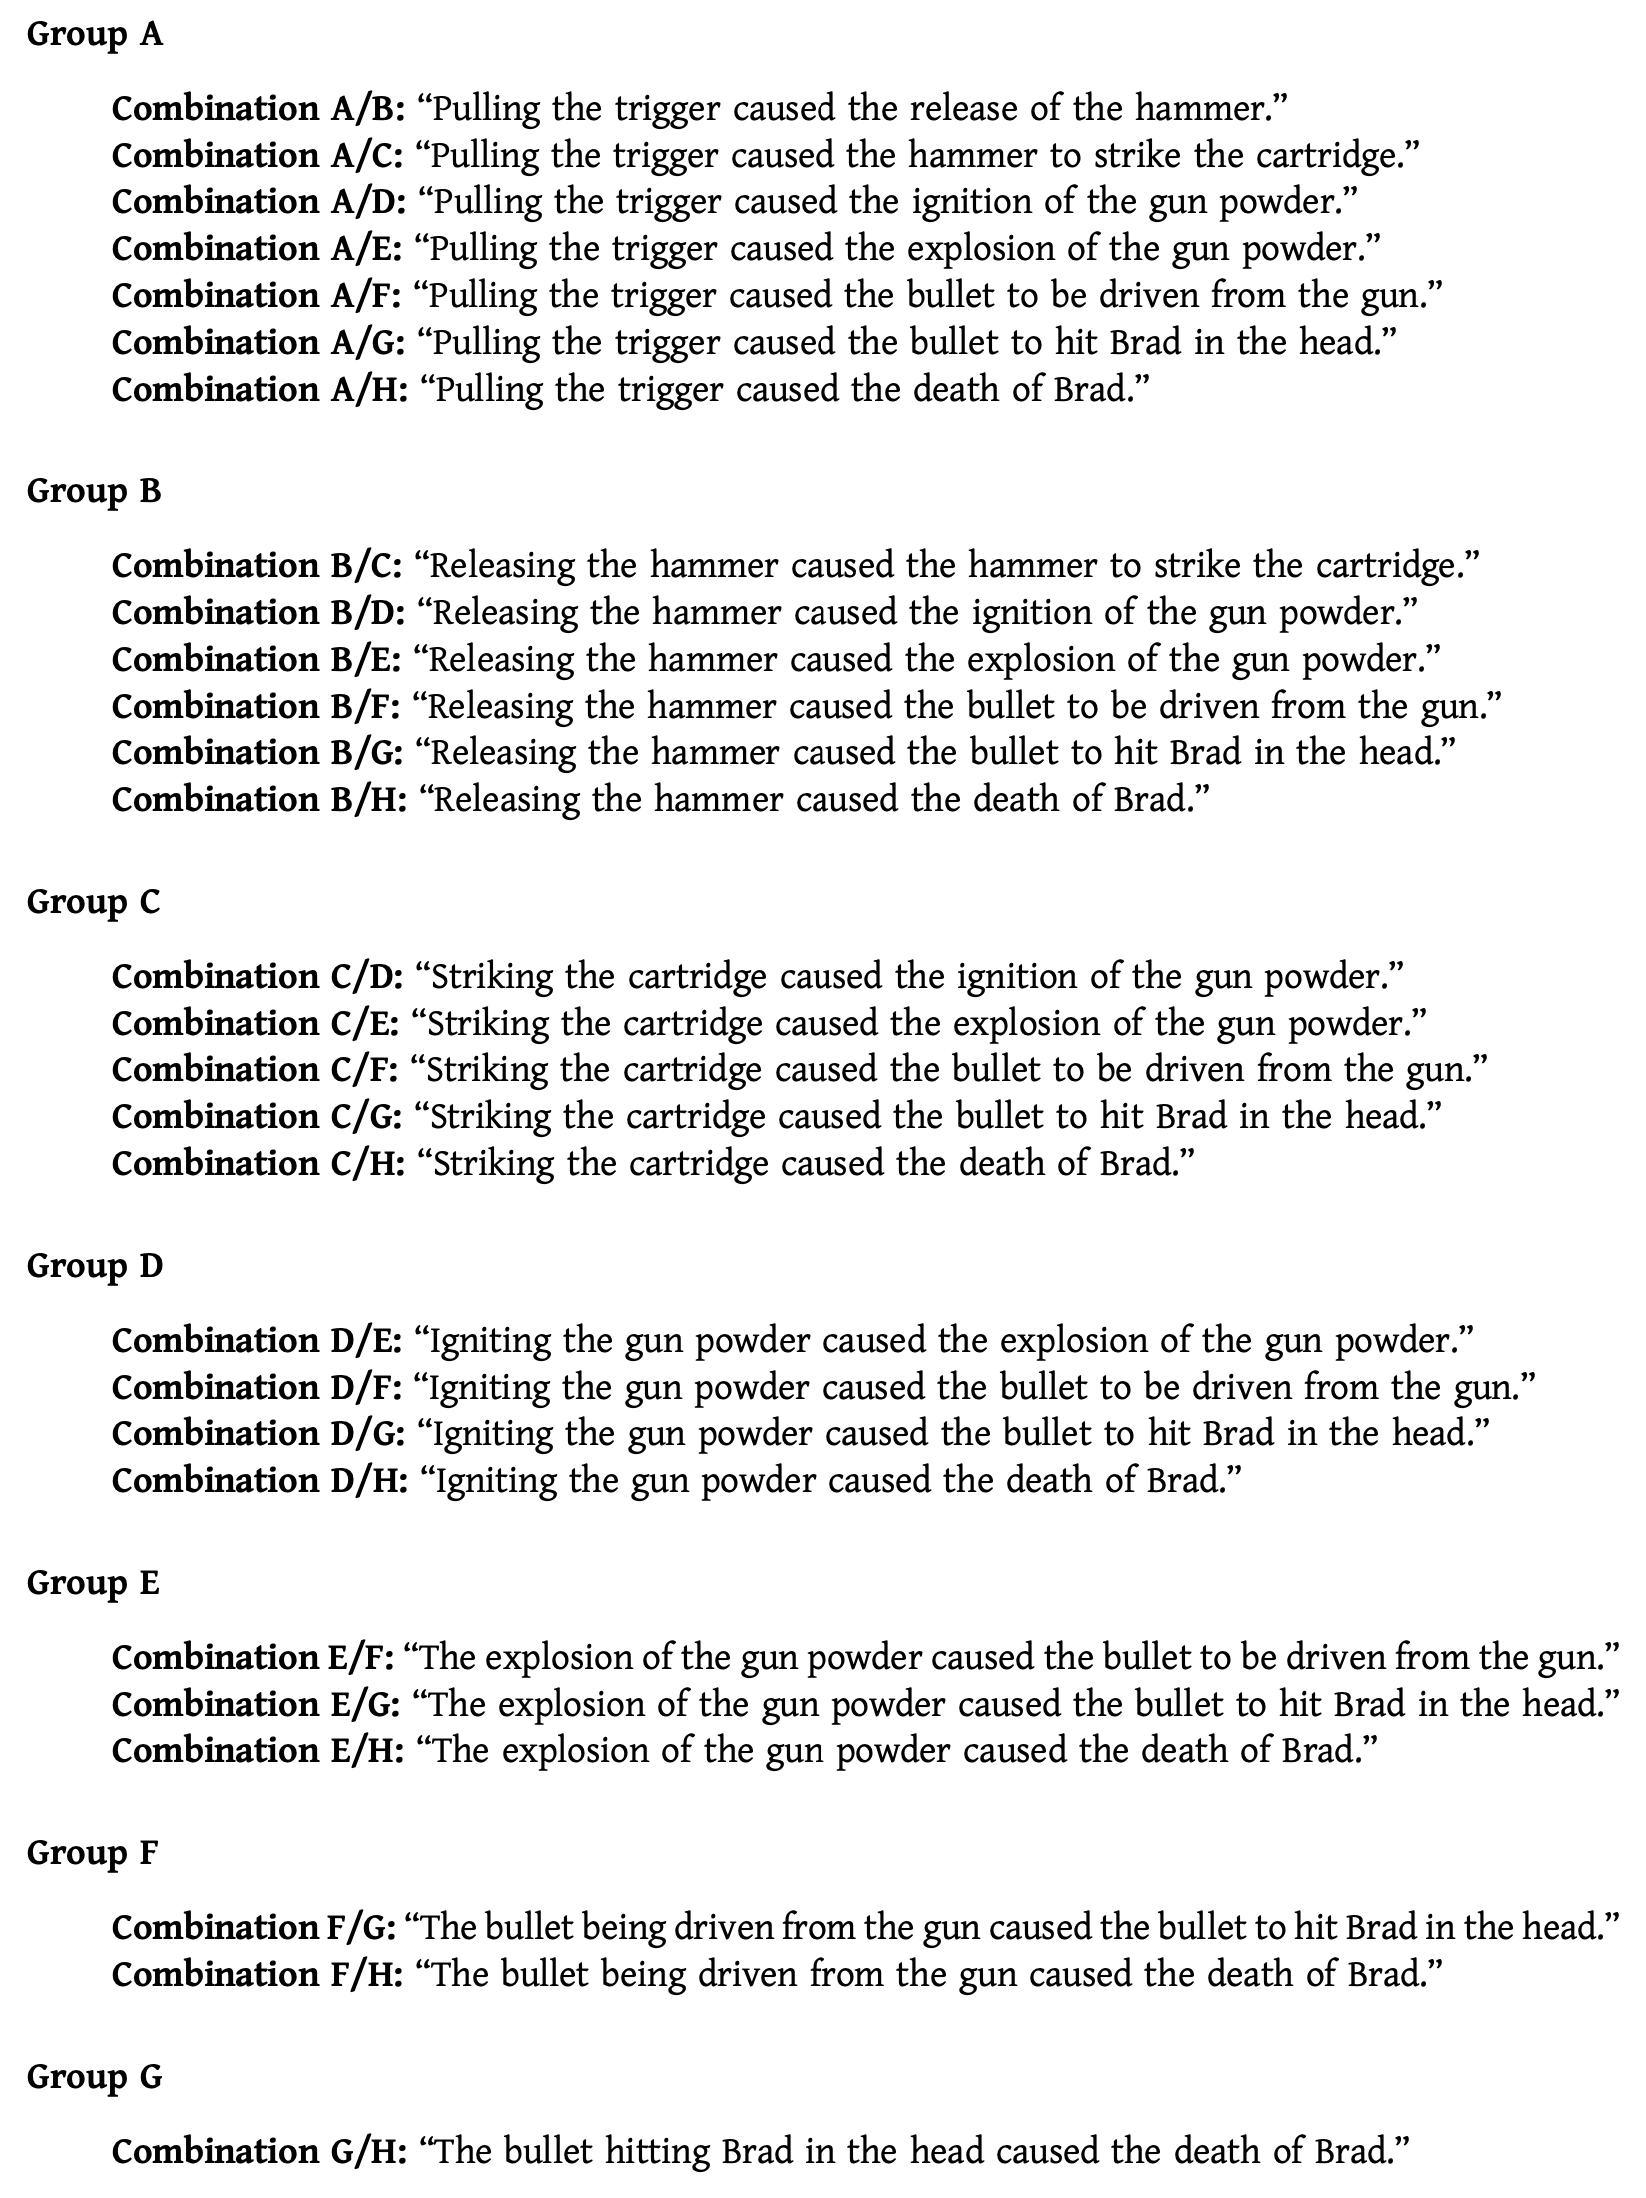
\includegraphics[width=0.35\linewidth]{figures/bauer_romann_2020_app_a.png}}\\
   {\footnotesize\textbf{Appendix A:} Items}\\
\end{center}
\end{frame}


%%%%%%%%%%%%
% SLIDE 21 %
%%%%%%%%%%%%
\begin{frame}{\vspace*{10mm}Bauer and Romann (2022): ``Answers at Gunpoint''}
\vspace*{-5mm}
\begin{multicols}{2}
\begin{center}
   \frame{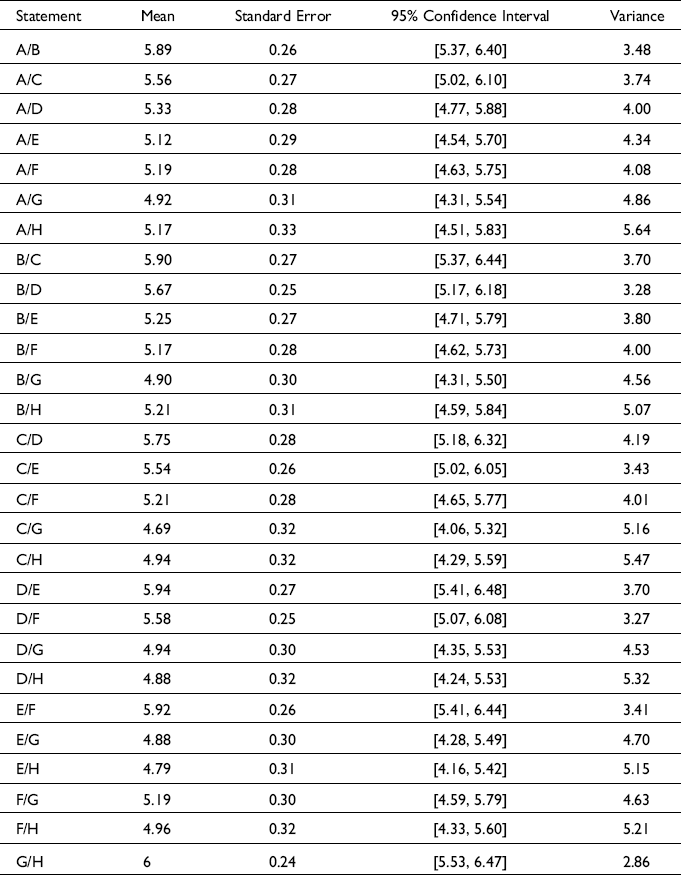
\includegraphics[width=0.5\linewidth]{figures/bauer_romann_2020_tab_1.png}}\\
   {\footnotesize\textbf{Table 1:} Summary of statements}\\
   \frame{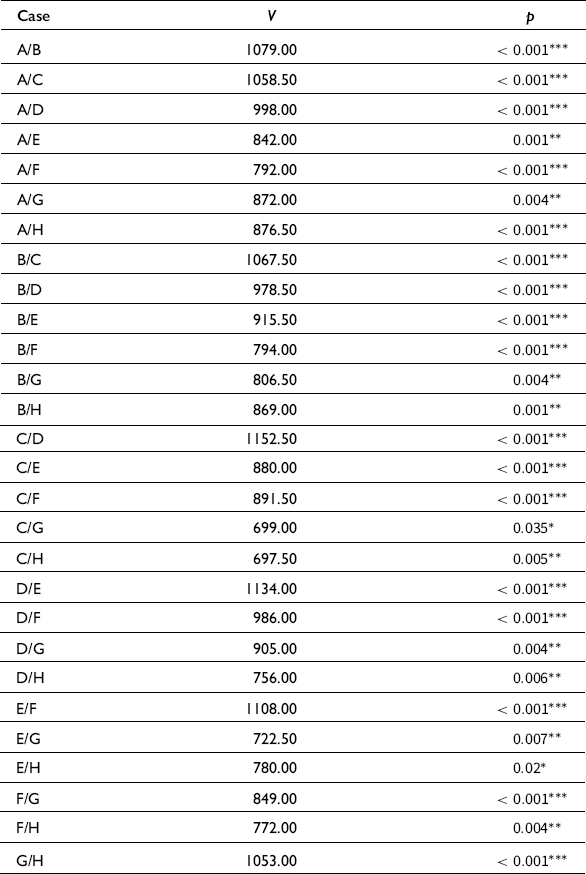
\includegraphics[width=0.5\linewidth]{figures/bauer_romann_2020_tab_2.png}}\\
   {\footnotesize\textbf{Table 2:} Two-tailed Wilcoxon signed-rank tests}
\end{center}
\end{multicols}
\end{frame}


%%%%%%%%%%%%
% SLIDE 22 %
%%%%%%%%%%%%
\begin{frame}{\vspace*{10mm}Bauer and Kornmesser (2023): ``Poisoned Babies, Shot Fathers, and Ruined Experiments''}
\vspace*{-5mm}
\begin{center}
   \frame{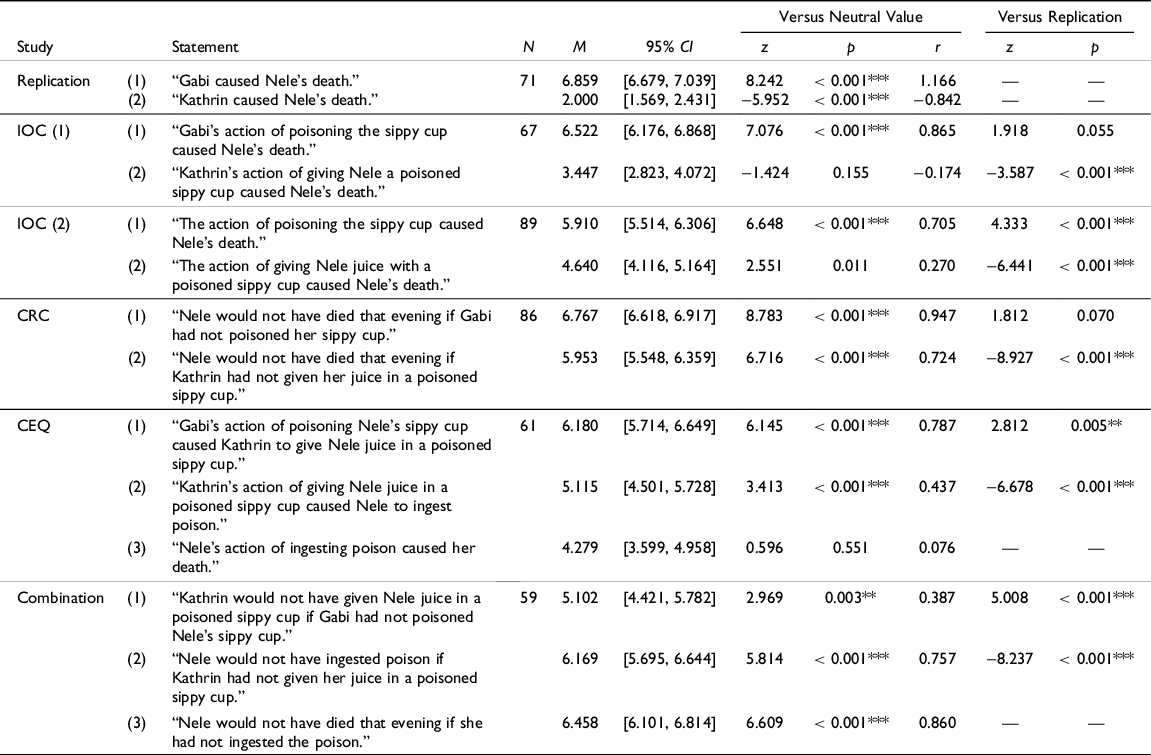
\includegraphics[width=0.5\linewidth]{figures/bauer_kornmesser_2023_tab_1}}\\
   {\footnotesize\textbf{Table 1:} Summary of statements for the poisoned cup vignette,\\reporting results of Wilcoxon signed-rank tests}
\end{center}
\end{frame}


%%%%%%%%%%%%
% SLIDE 23 %
%%%%%%%%%%%%
\begin{frame}{\vspace*{10mm}Bauer and Kornmesser (2023): ``Poisoned Babies, Shot Fathers, and Ruined Experiments''}
\vspace*{-5mm}
\begin{center}
   \frame{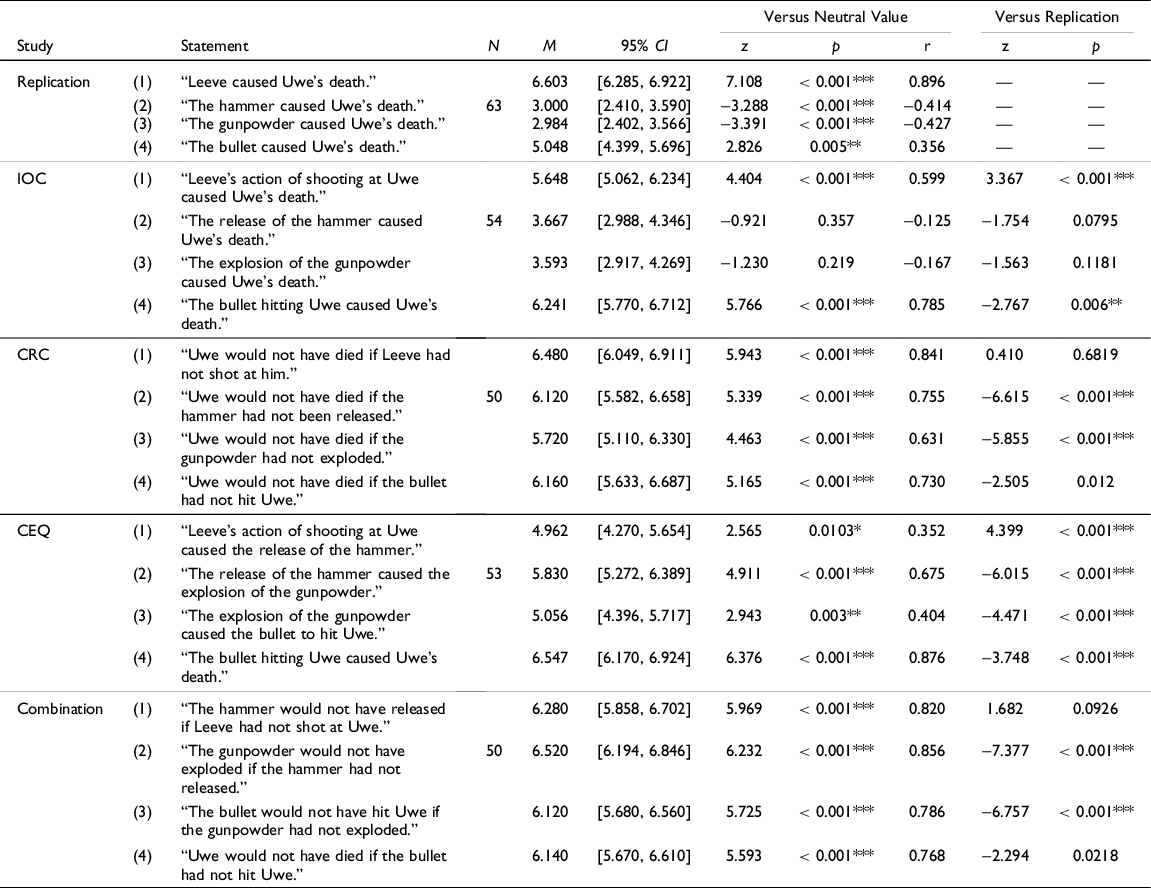
\includegraphics[width=0.5\linewidth]{figures/bauer_kornmesser_2023_tab_2}}\\
   {\footnotesize\textbf{Table 2:} Summary of statements for the revolver vignette,\\reporting results of Wilcoxon signed-rank tests}
\end{center}
\end{frame}


%%%%%%%%%%%%
% SLIDE 24 %
%%%%%%%%%%%%
\begin{frame}{\vspace*{10mm}Bauer and Kornmesser (2023): ``Poisoned Babies, Shot Fathers, and Ruined Experiments''}
\vspace*{-5mm}
\begin{center}
   \frame{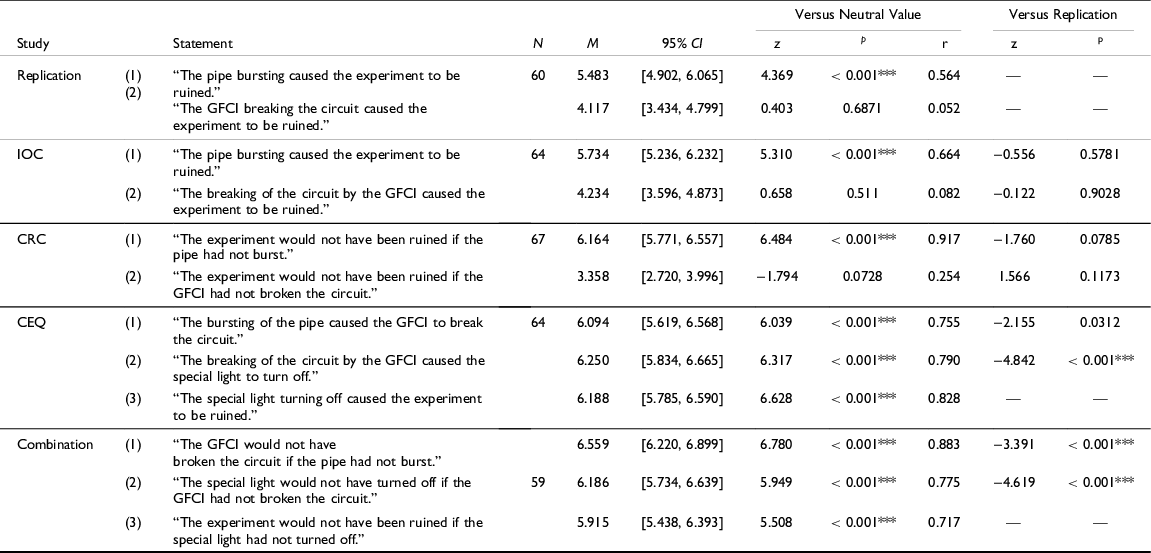
\includegraphics[width=0.5\linewidth]{figures/bauer_kornmesser_2023_tab_3}}\\
   {\footnotesize\textbf{Table 3:} Summary of statements for the GFCI vignette,\\reporting results of Wilcoxon signed-rank tests}
\end{center}
\end{frame}

\end{document}
